% UF Sample ETD Main Document Fall 2014
% 28 October, 2016: Modified slightly by LianTze Lim (Overleaf) to compile without errors
\documentclass[12pt,final,CPage]{ufthesis}
% Preamble %

% Define Packages To be used and options %
% here you define all the packages you wish to use in your paper, the ones shown are not all necessary,
% but all have purpose and can be very useful, so leave these as default and add packages as necassary
\usepackage{graphicx}
%\usepackage[dvipdfmx]{graphicx}
\usepackage{amsmath}
\usepackage{amsthm}
\usepackage{algpseudocode}
\usepackage{tabularx}
\usepackage{url}
\usepackage[letterpaper,hmargin=1in,vmargin=1in]{geometry}
\usepackage{lscape}
\usepackage{hanging}
\usepackage{longtable}
\usepackage{amsfonts}
\usepackage{amssymb}
%\usepackage[cmss]{sfmath} % Comment this line to use Times New Roman Math Typeface
\usepackage[cmbright]{sfmath} % Comment this line to use Times New Roman Math Typeface
\usepackage{subfigure}
\usepackage{rotating}
\usepackage{calc}
\usepackage{setspace}
\usepackage{ufenumerate}
\usepackage{latexsym}
\usepackage{epsf}
\usepackage{epsfig}
\usepackage{euscript}
\usepackage[format=hang,justification=raggedright,singlelinecheck=0,labelsep=period]{caption}
%\usepackage[numbers,sort&compress]{natbib} %Use this set-up for numbered reference lists
\usepackage[authoryear]{natbib} %Use this set-up if you want an un-numbered reference list
%\usepackage{hypernat}



\usepackage[hyperfootnotes=false]{hyperref}
%\usepackage[dvipdfmx,hyperfootnotes=false]{hyperref}
%\usepackage[dvips,hyperfootnotes=false]{hyperref}
\hypersetup{colorlinks=true,linkcolor=blue,anchorcolor=blue,citecolor=blue,filecolor=blue,urlcolor=blue,bookmarksnumbered=true,pdfview=FitB} %
% % %DO NOT PLACE ANY PACKAGES AFTER THE HYPERREF SET UP


\def\UrlFont{\rmfamily} %use this line for Times New Roman
% \def\UrlFont{\sffamily} %use this line for CMSS

%\allowdisplaybreaks  % % This command allows equation arrays and similar environments
% % % to break across pages to improve text flow - use only if needed.

% Prevent figures, tables or algorithms from using a separate page or column alone
\renewcommand{\topfraction}{0.85}
\renewcommand{\textfraction}{0.1}
\renewcommand{\floatpagefraction}{0.75}

% *** Do not adjust lengths that control margins, column widths, etc. ***
% *** Do not use packages that alter fonts (such as pslatex).         ***
% There should be no need to do such things with IEEEtran.cls V1.6 and later.
% correct bad hyphenation here
%\hyphenation{op-tical net-works semi-C:\Program Files\MiKTeX 2.5\miktexconduc-tor}

%------------------------------------------%

% Extra commands or misc formatting such as page alignment or output paper-size commands

%\include{extraparameters}

%------------------------------------------%

% Set your personal and paper information
\SetFullName{Shawn David Taylor}%
\SetThesisType{Dissertation}%{Dissertation} %{Thesis}
\SetDegreeType{Doctor of Philosophy}% {Doctor of Philosophy} {Master of Science}
\SetGradMonth{December}%
\SetGradYear{2019}%
\SetDepartment{Interdisciplinary Ecology}%
\SetChair{Ethan P. White}%
%\SetCochair{John W. Carver III}%uncomment this line and enter the name of your cochair inside the braces if you have one.
%If you have a cochair there two places in the ufthesis.cls file that will need to be uncommented as well
%In the "getting personal information" section about line 630
%And the "Abstract" Section around line 556
% Type your title here in all CAPS %
\SetTitle{FORECASTING PLANT PHENOLOGY: AN ASSESSMENT OF DATA SOURCES AND ESTIMATORS, AND A FULLY AUTOMATED IMPLEMENTATION}



% Define student-specific info (self-explanatory) %
%\include{userinfo}

%------------------------------------------%

% user defined commands in order to geC:\Program Files\MiKTeX 2.5\miktexnerate new commands, macros, and redefine default commands %
% user defined commands %
% Here is where you define optional commands such as macros, new commands,
% and new environments to be used in your paper

% optional command to prevent a word from breaking across a line %
\hyphenchar\font=-1


% Commands to produce proper bullet list
\newlength{\widthOfItem}
\let\Itemize=\itemize
\let\endItemize=\enditemize
\renewenvironment{itemize}{%
	\begin{Itemize}
		\setlength{\itemsep}{0.5\baselineskip}
		\setlength{\labelwidth}{2em}
		\setlength{\listparindent}{.32in}%
		\setlength{\leftmargin}{.32in}
		\setlength{\rightmargin}{0in}
		\settowidth{\widthOfItem}{\labelitemi}
		\setlength{\labelsep}{\leftmargin-\widthOfItem}
		\renewcommand{\labelitemii}{--}
		\singlespacing}{%
	\end{Itemize}}

% shortcut for setting up inserting \prime command in mathmode to avoid errors %
\newcommand{\p}{^{\prime}}

% shortcuts for prime color text
\newcommand{\red}{\textcolor[rgb]{1.00,0.00,0.00}}
\newcommand{\green}{\textcolor[rgb]{0.00,1.00,0.00}}
\newcommand{\blue}{\textcolor[rgb]{0.00,0.00,1.00}}

% Shorcut commands for mathmatical formulas %

\newcommand{\latex}{\LaTeX 2\ensuremath{\epsilon}}

% THEOREM Environments ---------------------------------------------------
%These environments are provided as a convenience - feel free to modify if needed

\newtheorem{theorem}{Theorem}[chapter]%To link the theorem to each chapter uncomment the chapter option
\newtheorem{lemma}{Lemma}%[theorem]% To link each lemma to a theorem uncomment the theorem option
\newtheorem{corollary}{Corollary}%[theorem]% To link each corollary to a theorem uncomment the theorem option
% to link a corollary to a chapter change the theorem option to chapter
\newtheorem{definition}{Definition}%[chapter] %the same is true for both definitions and assumptions
\newtheorem{assumption}{Assumption}%[chapter] %
\newtheorem{proposition}{Proposition}[chapter]
\newtheorem{algorithm}{Algorithm}[chapter]


%These were some user commands I've run across that I thought some might want to incorporate into their work
%\newcommand{\bdm}{
 %   \begin{displaymath}}

%\newcommand{\edm}{
%    \end{displaymath}}

%\newcommand{\be}{
%    \begin{equation}}

%\newcommand{\ee}{
%    \end{equation}}

%\newcommand{\bea}{
 %   \begin{eqnarray}}

%\newcommand{\eea}{
%    \end{eqnarray}}


%-------------------------------------------------------------------------------------------------------%

% Begin Main Part of Document %

\begin{document}


 % % % % % % % % % % % % % % % % % % % % % % % % % % % % % % % % % % % % % %
 % Remember - You MUST get a .bst file that matches the Journal in your
 % field that you choose as your Reference example
 % NONE of these examples will satisfy the Graduate Editorial Office
 % if they don't match your Journal example!!!!
 % NOTE: If you use a numbered reference system and your references
 % are set in parentheses rather than brackets you need to select the
 % Natbib option "numbers sort and compress" in the packages.tex file
 % % % % % % % % % % % % % % % % % % % % % % % % % % % % % % % % % % % % % %


 %Note that the path separator is a forward slash NOT a back slash
 %Place YOUR .bst file in the bst folder and use that filename (without the .bst extension)
 % as your Bibliography Style file

%\bibliographystyle{bst/abbrv}
%\bibliographystyle{bst/abbrvnat}
%\bibliographystyle{bst/abbrvurl_uf}
%\bibliographystyle{bst/alphaurl_uf}
%\bibliographystyle{bst/apa-good}
%\bibliographystyle{bst/Chicago_Web}
\bibliographystyle{bst/ecology_web}
%\bibliographystyle{bst/IEEEtran}
%\bibliographystyle{bst/mla_web}
%\bibliographystyle{bst/mla-good}
%\bibliographystyle{bst/plainnat}
%\bibliographystyle{bst/plainurl_uf}
%\bibliographystyle{bst/Science_Web}
%\bibliographystyle{bst/uf_econ}
%\bibliographystyle{bst/uffull}
%\bibliographystyle{bst/ufinit}
%\bibliographystyle{bst/unsrtnat}
%\bibliographystyle{bst/unsrturl_uf}
%\bibliographystyle{bst/plain}
%\bibliographystyle{bst/ufinit}
%\bibliographystyle{bst/plainurl_uf}


%-----------------------------------------------------------------------%

\maketitle % % % % Creates the Title page from the information entered in userinfo.tex
\makecopyright

%------------------------------------------%

\dedication{% Add your text for the dedication here between the center tags
\addvspace{4.25in}
\begin{center}\singlespacing
I dedicate this dissertation to my family and friends around the world.\\
\end{center}
} % %Creates the dedication - if your dedication is more than a single line
% % % % % % % % % % % % % % % % % %you will need to reduce the vspace amount to keep the text centered verticlly
% % % % % % % % % % % % % % % % % %optional - comment or delete if you are not dedicating to anyone,

%------------------------------------------%

% Make sure to keep the text within the brackets and the output should turn out correct
\acknowledge{%
Thank you to my advisor, Ethan White, for all his help and motivation these past four years. Thanks to the members of the Weecology Lab. Thank you to my friends and family.}
 % % % %Required - There is no requirement to acknowledge a particular person
% % % % % % % % % % % % % % % % %but you must acknowledge someone (funding source, committee chair, spouse)?

%------------------------------------------%

% This file includes the file which creates the table of contents %
% This creates your table of contents, list of figures, and list of tables
% the pdfbookmark line adds the word to the bookmarks of the pdf without adding it to the TOC itself
\pdfbookmark[0]{TABLE OF CONTENTS}{tableofcontents}
\tableofcontents %
\listoftables %
%\setcounter{lofdepth}{2}
\listoffigures %

% Produced list of abbreviations or symbols %
%\printindex[keylist]{KEY TO ABBREVIATIONS}{KEY TO ABBREVIATIONS}{}
%\printindex[mathlist]{KEY TO SYMBOLS}{KEY TO SYMBOLS}{%
%The list shown below gives a brief description of the major mathematical symbols defined in this work. For each
%symbol, the page number corresponds to the place where the symbol is first used.} %
 %This file creates the Table of Contents, List of Figures, and List of Objects (if any)
% % % % % % % %delete or comment the file you want to remove

%------------------------------------------%

%%This is an optional file. A list of abbreviations is NOT even suggested.
%%Best practice is to define the item the first time it is used in the document

%%%-----------List of Symbols, Nomenclature or Abbreviation--------

%% Please note: a list of Symbols, terms, acronyms, etc. is not usually the best practice.
%% More often you should simply define an abbreviation the first time it is used.
%% If you DO need to include a list like this please notice that it must be paginated manually
%% by breaking it up into page size tables. Longtable will not wrap the definition properly if
%% it extends to a second line and a similar issue is encountered when the tabbing environment
%% is used. If you have a better way of meeting the Editorial Office requirements I'd love to hear about it.

\chapter*{LIST OF SYMBOLS, NOMENCLATURE, OR ABBREVIATIONS} \addcontentsline{toc}{chapter}{LIST OF SYMBOLS} %Start
%writing here. This is optional.
\singlespacing
\begin{tabular}{l p{5in}} %if the terms in the first column are longer than 1.4 inches reduce the number 5 appropriately
$\sum$ & Denotes the summation of a series of terms\\
\\%This adds the single space between definitions (required)
$\bigcap$ & A really big bigcap\\
\\
fractal & A geometric pattern that is repeated at ever smaller
scales to produce irregular shapes and surfaces that cannot be represented by classical
geometry. Fractals are used especially in computer modeling of irregular patterns and structures in nature.}\\
\\
polynomial & (in one variable) an expression consisting of the sum of two
or more terms each of which is the product of a constant and a
variable raised to an integral power: $ax^2 + bx + c$ is a
polynomial, where $a, b,$ and $c$ are constants and $x$ is a
variable.}\\
\\
$\sum$ & Denotes the summation of a series of terms\\
\\
$\bigcap$ & A really big bigcap\\
\\
fractal & A geometric pattern that is repeated at ever smaller
scales to produce irregular shapes and surfaces that cannot be represented by classical
geometry. Fractals are used especially in computer modeling of irregular patterns and structures in nature.}\\
\\
polynomial & (in one variable) an expression consisting of the sum of two
or more terms each of which is the product of a constant and a
variable raised to an integral power: $ax^2 + bx + c$ is a
polynomial, where $a, b,$ and $c$ are constants and $x$ is a
variable.}\\
\\
$\sum$ & Denotes the summation of a series of terms\\
\\
$\bigcap$ & A really big bigcap\\
\\
fractal & A geometric pattern that is repeated at ever smaller
scales to produce irregular shapes and surfaces that cannot be represented by classical
geometry. Fractals are used especially in computer modeling of irregular patterns and structures in nature.}\\
\\
polynomial & (in one variable) an expression consisting of the sum of two
or more terms each of which is the product of a constant and a
variable raised to an integral power: $ax^2 + bx + c$ is a
polynomial, where $a, b,$ and $c$ are constants and $x$ is a
variable.}\\

\end{tabular}

\begin{tabular}{lp{5in}}
$\sum$ & Denotes the summation of a series of terms\\
\\
$\bigcap$ & A really big bigcap\\
\\
fractal & A geometric pattern that is repeated at ever smaller
scales to produce irregular shapes and surfaces that cannot be represented by classical
geometry. Fractals are used especially in computer modeling of irregular patterns and structures in nature.}\\
\\
polynomial & (in one variable) an expression consisting of the sum of two
or more terms each of which is the product of a constant and a
variable raised to an integral power: $ax^2 + bx + c$ is a
polynomial, where $a, b,$ and $c$ are constants and $x$ is a
variable.}\\
\\
$\sum$ & Denotes the summation of a series of terms\\
\\
$\bigcap$ & A really big bigcap\\
\\
fractal & A geometric pattern that is repeated at ever smaller
scales to produce irregular shapes and surfaces that cannot be represented by classical
geometry. Fractals are used especially in computer modeling of irregular patterns and structures in nature.}\\
\\
polynomial & (in one variable) an expression consisting of the sum of two
or more terms each of which is the product of a constant and a
variable raised to an integral power: $ax^2 + bx + c$ is a
polynomial, where $a, b,$ and $c$ are constants and $x$ is a
variable.}\\
\\
$\sum$ & Denotes the summation of a series of terms\\
\\
$\bigcap$ & A really big bigcap\\
\\
fractal & A geometric pattern that is repeated at ever smaller
scales to produce irregular shapes and surfaces that cannot be represented by classical
geometry. Fractals are used especially in computer modeling of irregular patterns and structures in nature.}\\
\\
polynomial & (in one variable) an expression consisting of the sum of two
or more terms each of which is the product of a constant and a
variable raised to an integral power: $ax^2 + bx + c$ is a
polynomial, where $a, b,$ and $c$ are constants and $x$ is a
variable.}\\
\\
\end{tabular}
\doublespacing




%------------------------------------------%
% This line adds the word CHAPTER to the TOC just before the listing of the chapter and subsections begins
\addtocontents{toc}{\protect\addvspace{10pt}\noindent{CHAPTER}\protect\hfill\par}{}% This extra line adds the word CHAPTER to the table of contents %
\phantomsection
% Write in only the text of your abstract, all the extra heading jargon is automatically taken care of
\begin{abstract}
Abstracts should be less than 350 words. Any Greek letters or symbols not found on a standard computer keyboard will have to be spelled out in the electronic version so try to avoid them in the Abstract if possible. The best way to compile the document is to use the make\_xelatex.bat file. If you are using Linux or Macintosh Operating Systems there are examples of make files for these systems in the Make Files Folder but they may be outdated and need to be modified for them to work properly. This document is the official tutorial outlining the use and implementation of the UF \LaTeX 2\ensuremath{\epsilon} Template for use on thesis and dissertations. The tutorial will cover the basic files, commands, and syntax in order to properly implement the template.  It should be made clear that this tutorial will not tell
one how to use \LaTeX 2\ensuremath{\epsilon}.  It will be assumed that you will have had some previous knowledge or experience with \LaTeX 2\ensuremath{\epsilon}, but, there are many aspects of publishing for the UF Graduate School that requires attention to some details that are normally not required in \LaTeX 2\ensuremath{\epsilon}.

Pay particular attention to the section on references. NONE of the bibliography style files (.bst) are an assurance that your document's reference style will meet the Editorial Guidelines. You MUST get a .bst file that matches the style used by the journal you used as a guide for your references and citations. The files included in this document are examples only and are NOT to be used unless they match your sample article exactly!

You should have a .bib file (we have included several examples) that contains your reference sources. Place your .bib file in the bib folder and enter the name of the file in the list of bib files, or enter your reference information into one of our existing .bib files if you don't already have one. Just make sure to preserve the format of each kind of reference. Each time you cite a reference you enter the "key" (the first field in the reference listing in the .bib file) associated with that reference. During the compilation process LaTeX will gather all the references, insert the correct method of citation and list the references in the correct location in the proper format for the reference style selected.
\end{abstract}
 %The abstract is created using this file and userinfo.tex
% % % % % % % % % % %If you have a c-chair you must uncomment that line in userinfo.tex AND find the
% % % % % % % % % % %co-chair lines in ufthesis.cls and un-comment those as well

%-----------------------------------------------------------------------%

% This section encompasses the main body of the paper from all the content through to the biographical sketch

% Chapters to be included (more can be added by creating a new chapter#.tex %
% file and then implementing the \inlcude{chapter#.tex} command as seen below %
\chapter{INTRODUCTION} \label{introduction}

Plant phenology, the timing of recurring biological events such as flowering, plays an important role in ecological research extending from local to global scales \citep{cleland2007, richardson2013, tang2016}. At large scales the timing of spring leaf out and fall senescence influence the carbon budget of earth system models, which has implications for correctly accounting for biosphere-atmosphere feed backs in long-term climate forecasts \citep{richardson2012}. At smaller scales, species-specific responses to temperature and precipitation can alter flower communities \citep{diez2012, caradonna2014, theobald2017} and affect the abundance and richness of both pollinators \citep{ogilvie2017a, ogilvie2017b} and organisms at higher trophic levels \citep{tylianakis2008}. 

Because of the central importance of phenology, advanced forecasts for when phenological events will occur have numerous potential applications including: 1) research on the cascading effects of changing plant phenology on other organisms; 2) tourism planning related to flower blooms and autumn colors; 3) planning for sampling and application of management interventions by researchers and managers; and 4) agricultural decisions on timing for planting, harvesting, and application of pest prevention techniques. However, due to the challenges of automatically integrating, predicting, and disseminating large volumes of data, there are limited examples of applied phenology forecast systems. Plant phenology models that are robust at multiple ecological scales, or deemed appropriate for a particular scale, are needed to better understand and forecast the timing of key biological events. Additionally, phenology data at a suitable spatial extent has only recently come online and poses several challenges for validation and integration into phenological models. 

Plant phenology models have historically been parameterized using data from long-term, well-sampled study sites. Yet data from a single location might not be suitable for large-scale phenology forecasts. Large-scale data is available, but comes from citizen science programs where several potentially biases can be introduced \citep{dickinson2010}. A thorough evaluation of the data capability is needed before integrating citizen science data into the pipeline for a plant phenology forecast. Data validation will ensure that any potential biases in the phenological observations are either non-existent, or too small to affect phenological models. 

The variable of interest in plant phenology models is the transition date. For example the date a flower blooms or leaf emerges is the onset transition date. Other common transition dates are first observed open flowers or new leafs on a plant, but can also include peak flower, fruit maturation, and leaf senescence. Historic datasets often use repeated observations to identify the true transition date  \citep{davis2015, wolkovich2012}, yet this is susceptible to observer bias  \citep{miller-rushing2008}. Most modern studies and collection protocols use status-based monitoring, where observers record the current state of a plant (ie. leaves present or absent) without necessarily conducting repeated observations to observe recent or future transitions. This includes research using herbarium records, where the presence or absence of flowers and other phenophases is inferred from their presence on a specimen  \citep{willis2017}. To make use of status-based data in most phenological models the transition date must first be estimated, and to date few comprehensive comparison of these estimators have been performed. Here I perform an evaluation of several transition date estimators using an 11 year observational dataset. 

Large-scale forecast systems are are complex pipelines which ingest, process, and combine several continuous streams of data. The knowledge acquired and lessons learned in building these systems will help define best practices and needed tools and training for other groups to implement similar systems \citep{yenni2019}. A thorough description of the pipeline, and the challenges which were overcome in building it, will help advance the field of ecological forecasting. This pipeline description, along with validation of phenological data, are the first steps in implementing a continuously updated phenology forecast system. 



\chapter{LITERATURE REVIEW} \label{lit}

\section{Dolor Sit Amet}

 Many of the problems in theses and dissertations involve tables. The UF Graduate Counsel is very specific in the Table Requirements. There should be no vertical lines in tables and only three horizontal lines. No bold text, etc., see the web site for the complete list of requirements. One simple improvement can be incorporated by using tabularx instead of the tabular environment. This allows a table to be stretched the full text width easily, which avoids the centered or left aligned issue. Table \ref{first} is an examble of the tabularx code. Consectetur adipiscing elit. Fusce eget tempus lectus, non porttitor tellus. Aliquam molestie sed urna quis convallis. Aenean nibh eros, aliquam non eros in, tempus lacinia justo. In magna sapien, blandit a faucibus ac, scelerisque nec purus.
 
 \begin{table}[htbp]
    \caption{A sample Table}\label{first}
    \begin{tabularx}{6.5in}{XXX}
      \hline
      First & Second & Third \\
      \hline
      12 & 45 & 26 \\
      17 & 32 & 93 \\
      text & 51 & can be there too. \\	
      \epsfig{figure=images/cat.eps, scale=1} & 28 & Figures too - a cat. \\
      \begin{turn}{0}\epsfig{figure=images/mouse.eps, scale=0.25}\end{turn} & 000 & and a mouse! \\
      \hline
    \end{tabularx}
\end{table}
 
 
 Praesent fermentum felis nec massa interdum, vel dapibus mi luctus. Cras id fringilla mauris. Ut molestie eros mi, ut hendrerit nulla tempor et. Pellentesque tortor quam, mattis a scelerisque nec, euismod et odio. Mauris rhoncus metus sit amet risus mattis, eu mattis sem interdum.

\subsection{Platea Dictumst}
Donec convallis scelerisque ante, in sollicitudin orci laoreet eu. Nam arcu magna, semper vel lorem eu, venenatis ultrices est. Nam aliquet ut erat ac scelerisque. Maecenas ut molestie mi. Phasellus ipsum magna, sollicitudin eu ipsum quis, imperdiet cursus turpis. Etiam pretium enim a fermentum accumsan. Morbi vel vehicula enim.


\subsection{Long (and/or Wide) Tables}

Another problem in LaTeX is the inability to handle long tables. While there are some packages that address this problem none of them quite fit the Editorial Office guidelines. The caption is not repeated but we do need "Table x-y. Continued" on each subsequent page and a repeat of the column headings on each page as well. The following table is the best example of the correct format I can produce. The disadvantage of this method is that much of it is manually set up and changes in the text will cause changes in the table. \citep{Moffatt69} For best results avoid the use of footnotemark and footnotetext commands inside of tables and try to keep your footnotes outside of floats whenever possible.



\begin{table}
\caption{Feasible triples for highly variable Grid, MLMMH.} \label{tbl1}
\begin{tabularx}{6.5 in}{r l X}
\hline {{Time (s)}} & {{Triple chosen}} & {{Other feasible triples}} \\ \hline
0 & (1, 11, 13725) & (1, 12, 10980), (1, 13, 8235), (2, 2, 0), (3, 1, 0) \\
2745 & (1, 12, 10980) & (1, 13, 8235), (2, 2, 0), (2, 3, 0), (3, 1, 0) \\
5490 & (1, 12, 13725) & (2, 2, 2745), (2, 3, 0), (3, 1, 0) \\
8235 & (1, 12, 16470) & (1, 13, 13725), (2, 2, 2745), (2, 3, 0), (3, 1, 0) \\
10980 & (1, 12, 16470) & (1, 13, 13725), (2, 2, 2745), (2, 3, 0), (3, 1, 0) \\
13725 & (1, 12, 16470) & (1, 13, 13725), (2, 2, 2745), (2, 3, 0), (3, 1, 0) \\
16470 & (1, 13, 16470) & (2, 2, 2745), (2, 3, 0), (3, 1, 0) \\
19215 & (1, 12, 16470) & (1, 13, 13725), (2, 2, 2745), (2, 3, 0), (3, 1, 0) \\
21960 & (1, 12, 16470) & (1, 13, 13725), (2, 2, 2745), (2, 3, 0), (3, 1, 0) \\
24705 & (1, 12, 16470) & (1, 13, 13725), (2, 2, 2745), (2, 3, 0), (3, 1, 0) \\
27450 & (1, 12, 16470) & (1, 13, 13725), (2, 2, 2745), (2, 3, 0), (3, 1, 0) \\
30195 & (2, 2, 2745) & (2, 3, 0), (3, 1, 0) \\
32940 & (1, 13, 16470) & (2, 2, 2745), (2, 3, 0), (3, 1, 0) \\
35685 & (1, 13, 13725) & (2, 2, 2745), (2, 3, 0), (3, 1, 0) \\
38430 & (1, 13, 10980) & (2, 2, 2745), (2, 3, 0), (3, 1, 0) \\
41175 & (1, 12, 13725) & (1, 13, 10980), (2, 2, 2745), (2, 3, 0), (3, 1, 0) \\
43920 & (1, 13, 10980) & (2, 2, 2745), (2, 3, 0), (3, 1, 0) \\
46665 & (2, 2, 2745) & (2, 3, 0), (3, 1, 0) \\
49410 & (2, 2, 2745) & (2, 3, 0), (3, 1, 0) \\
52155 & (1, 12, 16470) & (1, 13, 13725), (2, 2, 2745), (2, 3, 0), (3, 1, 0) \\
54900 & (1, 13, 13725) & (2, 2, 2745), (2, 3, 0), (3, 1, 0) \\
57645 & (1, 13, 13725) & (2, 2, 2745), (2, 3, 0), (3, 1, 0) \\
60390 & (1, 12, 13725) & (2, 2, 2745), (2, 3, 0), (3, 1, 0) \\
63135 & (1, 13, 16470) & (2, 2, 2745), (2, 3, 0), (3, 1, 0) \\
65880 & (1, 13, 16470) & (2, 2, 2745), (2, 3, 0), (3, 1, 0) \\
68625 & (2, 2, 2745) & (2, 3, 0), (3, 1, 0) \\
71370 & (1, 13, 13725) & (2, 2, 2745), (2, 3, 0), (3, 1, 0) \\
74115 & (1, 12, 13725) & (2, 2, 2745), (2, 3, 0), (3, 1, 0) \\
76860 & (1, 13, 13725) & (2, 2, 2745), (2, 3, 0), (3, 1, 0) \\
79605 & (1, 13, 13725) & (2, 2, 2745), (2, 3, 0), (3, 1, 0) \\
82350 & (1, 12, 13725) & (2, 2, 2745), (2, 3, 0), (3, 1, 0) \\
85095 & (1, 12, 13725) & (1, 13, 10980), (2, 2, 2745), (2, 3, 0), (3, 1, 0) \\
87840 & (1, 13, 16470) & (2, 2, 2745), (2, 3, 0), (3, 1, 0) \\
90585 & (1, 13, 16470) & (2, 2, 2745), (2, 3, 0), (3, 1, 0) \\
93330 & (1, 13, 13725) & (2, 2, 2745), (2, 3, 0), (3, 1, 0) \\
96075 & (1, 13, 16470) & (2, 2, 2745), (2, 3, 0), (3, 1, 0) \\
98820 & (1, 13, 16470) & (2, 2, 2745), (2, 3, 0), (3, 1, 0) \\
101565 & (1, 13, 13725) & (2, 2, 2745), (2, 3, 0), (3, 1, 0) \\
104310 & (1, 13, 16470) & (2, 2, 2745), (2, 3, 0), (3, 1, 0) \\
107055 & (1, 13, 13725) & (2, 2, 2745), (2, 3, 0), (3, 1, 0) \\
109800 & (1, 13, 13725) & (2, 2, 2745), (2, 3, 0), (3, 1, 0) \\
112545 & (1, 12, 16470) & (1, 13, 13725), (2, 2, 2745), (2, 3, 0), (3, 1, 0) \\
\hline
\end{tabularx}
\end{table}

\begin{table}[h!t!]
\begin{tabularx}{6.5 in}{r l X}
\multicolumn{3}{l}{Table \ref{tbl1}. Continued}\\%
\hline {{Time (s)}} & {{Triple chosen}} & {{Other feasible triples}} \\ \hline
115290 & (1, 13, 16470) & (2, 2, 2745), (2, 3, 0), (3, 1, 0) \\
118035 & (1, 13, 13725) & (2, 2, 2745), (2, 3, 0), (3, 1, 0) \\
120780 & (1, 13, 16470) & (2, 2, 2745), (2, 3, 0), (3, 1, 0) \\
123525 & (1, 13, 13725) & (2, 2, 2745), (2, 3, 0), (3, 1, 0) \\
126270 & (1, 12, 16470) & (1, 13, 13725), (2, 2, 2745), (2, 3, 0), (3, 1, 0) \\
129015 & (2, 2, 2745) & (2, 3, 0), (3, 1, 0) \\
131760 & (2, 2, 2745) & (2, 3, 0), (3, 1, 0) \\
134505 & (1, 13, 16470) & (2, 2, 2745), (2, 3, 0), (3, 1, 0) \\
137250 & (1, 13, 13725) & (2, 2, 2745), (2, 3, 0), (3, 1, 0) \\
139995 & (2, 2, 2745) & (2, 3, 0), (3, 1, 0) \\
142740 & (2, 2, 2745) & (2, 3, 0), (3, 1, 0) \\
145485 & (1, 12, 16470) & (1, 13, 13725), (2, 2, 2745), (2, 3, 0), (3, 1, 0)\\%
148230 & (2, 2, 2745) & (2, 3, 0), (3, 1, 0) \\
150975 & (1, 13, 16470) & (2, 2, 2745), (2, 3, 0), (3, 1, 0) \\
153720 & (1, 12, 13725) & (2, 2, 2745), (2, 3, 0), (3, 1, 0) \\
156465 & (1, 13, 13725) & (2, 2, 2745), (2, 3, 0), (3, 1, 0) \\
159210 & (1, 13, 13725) & (2, 2, 2745), (2, 3, 0), (3, 1, 0) \\
161955 & (1, 13, 16470) & (2, 2, 2745), (2, 3, 0), (3, 1, 0) \\
164700 & (1, 13, 13725) & (2, 2, 2745), (2, 3, 0), (3, 1, 0) \\
\hline
\end{tabularx}
\end{table}

\section{Ex id ullamcorper commodo}
Augue sapien mattis leo, nec accumsan turpis quam at neque. Ut pellentesque velit sed placerat cursus. Integer congue urna non massa dictum, a pellentesque arcu accumsan. Nulla posuere, elit accumsan eleifend elementum, ipsum massa tristique metus, in ornare neque nisl sed odio. Nullam eget elementum nisi. Duis a consectetur erat, sit amet malesuada sapien. Aliquam nec sapien et leo sagittis porttitor at ut lacus. Vivamus vulputate elit vitae libero condimentum dictum. Nulla facilisi. Quisque non nibh et massa ullamcorper iaculis.

Integer laoreet bibendum arcu non pulvinar. Curabitur ac magna nibh. Phasellus sed nisi semper, molestie neque at, tempus lacus. Aenean vitae lacinia est. Phasellus aliquam lacus sit amet placerat molestie. Sed sit amet bibendum lectus, ac ornare ligula. Curabitur porttitor interdum tortor a dignissim. Quisque a placerat nibh. Phasellus lobortis imperdiet augue, non congue est bibendum eu. Vivamus tincidunt quam eu fringilla laoreet.

Maecenas efficitur dolor et ipsum convallis, ut fringilla neque luctus. Donec ac nisl quis leo gravida accumsan sit amet sed tellus. Quisque placerat hendrerit augue sit amet aliquet. Vestibulum laoreet consequat nunc, et egestas nisl auctor et. Duis scelerisque vulputate placerat. Proin tempus ligula ac tempor eleifend. Nullam est odio, commodo quis nisl eu, feugiat efficitur purus.

Duis egestas in mauris vel efficitur. Sed a faucibus sem, non euismod enim. Maecenas nec nulla justo. Suspendisse ut orci ac mi aliquet tincidunt ac eget quam. Quisque ac mi sagittis, dapibus dui a, facilisis neque. Aenean euismod orci sem, non imperdiet ipsum pulvinar ac. Proin eu vestibulum magna, eu ullamcorper nulla. Etiam enim felis, dignissim eget commodo ac, faucibus nec justo. Nulla condimentum velit imperdiet ligula aliquam semper. Nulla facilisi. Ut in lobortis metus, at dictum ipsum. Suspendisse facilisis nec eros eget mollis. Vestibulum eget dolor ac mauris lobortis gravida. Suspendisse consectetur orci in risus pharetra, sed eleifend nisl lacinia. Mauris augue nibh, commodo sed sem at, congue molestie massa. Suspendisse sodales aliquet tellus, a tristique nunc aliquam id.


\chapter{MATERIALS ANS METHODS} \label{materials}

\section{Consectetur Adipiscing Elit}

 Fusce eget tempus lectus, non porttitor tellus. Aliquam molestie sed urna quis convallis. Aenean nibh eros, aliquam non eros in, tempus lacinia justo. In magna sapien, blandit a faucibus ac, scelerisque nec purus. Praesent fermentum felis nec massa interdum, vel dapibus mi luctus. Cras id fringilla mauris. Ut molestie eros mi, ut hendrerit nulla tempor et. Pellentesque tortor quam, mattis a scelerisque nec, euismod et odio. Mauris rhoncus metus sit amet risus mattis, eu mattis sem interdum.

\subsection{This Is an Isolated Heading}
Either promote this to a section heading, add another subsection heading, or delete this heading.

\section{Augue sapien mattis leo}
Nec accumsan turpis quam at neque. Ut pellentesque velit sed placerat cursus. Integer congue urna non massa dictum, a pellentesque arcu accumsan. Nulla posuere, elit accumsan eleifend elementum, ipsum massa tristique metus, in ornare neque nisl sed odio. Nullam eget elementum nisi. Duis a consectetur erat, sit amet malesuada sapien. Aliquam nec sapien et leo sagittis porttitor at ut lacus. Vivamus vulputate elit vitae libero condimentum dictum. Nulla facilisi. Quisque non nibh et massa ullamcorper iaculis.


\chapter{AUTOMATED DATA-INTENSIVE FORECASTING OF PLANT PHENOLOGY THROUGHOUT THE UNITED STATES}

\section{Background}

Numerous phenology models have been developed to characterize the timing of major plant events and understand their drivers \citep{chuine2013}. These models are based on the idea that plant phenology is primarily driven by weather, with seasonal temperatures being the primary driver at temperate latitudes \citep{chuine2017, basler2016}. Because phenology is driven primarily by weather, it is possible to make predictions for the timing of phenology events based on forecasted weather conditions. The deployment of seasonal climate forecasts \citep{weisheimer2014}, those beyond just a few weeks, provides the potential to forecast phenology months in advance. This time horizon is long enough to allow meaningful planning and action in response to these forecasts. With well established models, widely available data, and numerous use cases, plant phenology is well suited to serve as an exemplar for near-term ecological forecasting. \renewcommand*{\thefootnote}{}\footnote{Reprinted with permission from Taylor, S.D. and White, E.P., 2019. Automated data-intensive forecasting of plant phenology throughout the United States. BioRxiv 634568 https://doi.org/10.1101/634568}

For decision making purposes, plant phenology forecasts would be most informative when produced at species- and phenophase-levels, over large spatial extents, and at fine spatial resolutions. Currently the only other plant phenology forecast is at a 1° lat/lon resolution, and uses a temperature based spring index which identifies when early-spring phenological events will occur \citep{schwartz2013, carrillo2018}. Forecasting at a higher level of detail is challenging due to the advanced computational tools needed for building and maintaining automatic forecasting systems \citep{welch2019, white2018}. Automated forecasts requires building systems that acquire data, make model-based predictions for the future, and disseminate the forecasts to end-users, all in an automated pipeline \citep{dietze2018, welch2019, white2018}. This is challenging even for relatively small-scale single site projects with one to several species or response variables due to the need for advanced computational tools to support robust automation \citep{welch2019, white2018}. Building an automated system to forecast phenology for numerous species at continental scales is even more challenging due to the large-scale data intensive nature of the analyses. Specifically, because phenology is sensitive to local climate conditions, phenology modeling and prediction should be done at high resolutions \citep{cook2010}. This requires repeatedly conducting computationally intensive downscaling of seasonal climate forecasts and making large numbers of predictions. To make 4 km resolution spatially explicit forecasts for the 78 species  in our study at continental scales requires over 90 million predictions for each updated forecast. To make the forecasts actionable these computational intensive steps need to be repeated in near real-time and disseminated in a way that allows end-users to understand the forecasts and their uncertainties \citep{dietze2018}.

Here we describe an automated near-term phenology forecast system we developed to make continental scale forecasts for 78 different plant species. Starting December 1st, and updated every 4 days, this system uses the latest climate information to make forecasts for multiple phenophases and presents the resulting forecasts and their uncertainty on a dynamic website, \href{https://phenology.naturecast.org/}{https://phenology.naturecast.org/}. Since the majority of plants complete budburst and/or flowering by the summer solstice in mid-June, this results in lead times off up to six months. We describe the key steps in the system construction, including: 1) fitting phenology models, 2) acquiring and downscaling climate data; 3) making predictions for phenological events; 4) disseminating those predictions; and 5) automating steps 2-4 to update forecasts at a sub-weekly frequency. We follow the framework of \cite{welch2019} for describing operationalized dynamic management tools (ie. self-contained tools running automatically and regularly) and describe the major design decisions and lessons learned from implementing this system that will guide improvements to automated ecological forecasting systems. Due to the data-intensive nature of forecasting phenology at fine resolutions over large scales this system serves as a model for large-scale forecasting systems in ecology more broadly. 

\section{Forecasting Pipeline}

\cite{welch2019} break down the process of developing tools for automated prediction into four stages: 1) Acquisition, obtaining and processing the regularly updated data needed for prediction; 2) Prediction, combining the data with models to estimate the outcome of interest; 3) Dissemination, the public presentation of the predictions; and 4) Automation, the tools and approaches used to automatically update the predictions using the newest data on a regular basis. We start by describing our approach to modeling phenology and then describe our approach to each of these stages.

\subsection{Phenology Modeling}

Making large spatial scale phenology forecasts for a specific species requires species level observation data from as much of its respective range as possible  \citep{taylor2018b}. We used data from the USA National Phenology Network (USA-NPN), which collects volunteer based data on phenological events and has amassed over 10 million observations representing over 1000 species. The USA-NPN protocol uses status-based monitoring, where observers answer yes, no, or unsure when asked if an individual plant has a specific phenophase present \citep{denny2014}. Phenophases refer to specific phases in the annual cycle of a plant, such as the presence of emerging leaves, flowers, fruit, or senescing leaves. We used the Individual Phenometrics data product, which provides pre-processed onset dates of individually monitored plants, for the phenophases budburst, flowering, and fall colors for all species with data between 2009 and 2017 \citep{npndata2017}. We only kept yes observations where the individual plant also had a no observation within the prior 30 days and dropped any records where a single plant had conflicting records for phenotype status or more than one series of yes observations for a phenophase in a 12 month period. We built models for species and phenophase combinations with at least 30 observations (Figure \ref{fig-4-1}-B) using daily mean temperature data at the location and time of each observation from the PRISM 4km dataset \citep{prismdata}. We also included contributed models of budburst, flowering, and/or fruiting for 5 species which were not well represented in the USA-NPN dataset (Table \ref{table-c-1}) \citep{prevey2019a, biederman2018}.

For each species and phenophase we fit an ensemble of four models using daily mean temperature as the sole driver (Figure \ref{fig-4-1}-C). The general model form assumes a phenological event will occur once sufficient thermal forcing units accumulate from a specified start day \citep{chuine2013, chuine2017}. The specification of forcing units are model specific, but all are derived from the 24-hour daily mean temperature. In a basic model a forcing unit is the maximum of either 0 or the mean temperature above 0°C (ie. growing degree days). The amount of forcing units required, and the date from which they start accumulating are parameterized for each species and phenophase (see Supplement for details). Ensembles of multiple models generally improve prediction over any single model by reducing bias and variance, and in a phenology context allow more accurate predictions to be made without knowing the specific physiological processes for each species \citep{basler2016, yun2017, dormann2018}. We used a weighted ensemble of four phenology models. We derived the weights for each model within the ensemble using stacking to minimize the root mean squared error on held out test data (100 fold cross-validation) as described in \cite{dormann2018} (see Supplement for details). After determining the weights we fit the core models a final time on the full dataset. Since individual process based phenology models are not probabilistic they do not allow the estimation of uncertainty in the forecasts. Therefore, we used the variance across the five climate models to represent uncertainty (see Prediction). Finally, we also fit a spatially corrected Long Term Average model for use in calculating anomalies (see Dissemination). This uses the past observations in a linear model with latitude as the sole predictor (see Supplement). 

In our pipeline 190 unique phenological models (one for each species and phenophase combination, see Table \ref{table-c-1}) needed to be individually parameterized, evaluated, and stored for future use. To consolidate all these requirements we built a dedicated software package written in Python, pyPhenology, to build, save, and load models, and also apply them to gridded climate datasets \citep{taylor2018a}. The package also integrates the phenological model ensemble so that the four sub-models can be treated seamlessly as one in the pipeline. After parameterizing each model, its specifications are saved in a text based JSON file that is stored in a git repository along with a metadata file describing all models (Figure \ref{fig-4-1}-D). This approach allows for the tracking and usage of hundreds of models, allowing models to be easily synchronized across systems, and tracking versions of models as they are updated (or even deleted).  

\subsection{Acquisition and Downscaling of Climate Data}

Since our phenology models are based on accumulated temperature forcing, making forecasts requires information on both observed temperatures (from Nov. 30 of the prior year up to the date a forecast is made) and forecast temperatures (from the forecast date onward). For observed data we used 4km 24-hour daily mean temperature from PRISM, a gridded climate dataset for the continental U.S.A. which interpolates on the ground measurements and is updated daily \citep{prismdata}. These observed data are saved in a netCDF file, which is appended with the most recent data every time the automated forecast is run. For climate forecasts we used the Climate Forecast System Version 2 (CFSv2;  a coupled atmosphere-ocean-land global circulation model) 2-m temperature data, which has a 6-hour timestep and a spatial resolution of 0.25 degrees latitude/longitude \citep{saha2014}. CFSv2 forecasts are projected out 9 months from the issue date and are updated every 6 hours. The five most recent climate forecasts are downloaded for each updated phenology forecast to accommodate uncertainty (see Prediction).

Because the gridded climate forecasts are issued at large spatial resolutions (0.25 degrees), this data requires downscaling to be used at ecologically relevant scales \citep{cook2010}. A downscaling model relates observed values at the smaller scale to the larger scale values generated by the climate forecast during a past time period. We regressed these past conditions from a climate reanalysis of CFSv2 from 1995-2015 \citep{saha2010} against the 4km daily mean temperature from the PRISM dataset for the same time period \citep{prismdata} to build a downscaling model using asynchronous regression (Figure \ref{fig-4-1}, E-G). The CFSv2 data is first interpolated from the original 0.25 degree grid to a 4km grid using distance weighted sampling, then an asynchronous regression model is applied to each 4km pixel and calendar month (see Appendix C for details) \citep{stoner2013}. The two parameters from the regression model for each 4 km cell are saved in a netCFD file by location and calendar month (Figure \ref{fig-4-1}-H). This downscaling model, at the scale of the continental U.S.A., is used to downscale the most recent CFSv2 forecasts to a 4km resolution during the automated steps. 

We used specialized Python packages to overcome the computational challenges inherent in the large CFSv2 climate dataset \citep{python}. The climate forecast data for each phenology forecast update is 10-40 gigabytes, depending on the time of year (time series are longer later in the year). While it is possible to obtain hardware capable of loading this dataset into memory, a more efficient approach is to perform the downscaling and phenology model operations iteratively by subsetting the climate dataset spatially and performing operations on one chunk at a time. We used the python package xarray \citep{xarray}, which allows these operations to be efficiently performed in parallel through tight integration with the dask package \citep{dask}. The combination of dask and xarray allows the analysis to be run on individual workstations, stand alone servers, and high performance computing systems, and to easily scale to more predictors and higher resolution data.

\subsection{Prediction}

The five most recent downscaled forecasts are each combined with climate observations to make a five member ensemble of daily mean temperature across the continental USA. These are used to make predictions using the phenology model for each species and phenophase (Figure \ref{fig-4-1}-M). Each climate ensemble member is a 3d matrix of latitude $\times$ longitude $\times$ time at daily timesteps extending from Nov. 1 of the prior year to 9 months past the issue date. The pyPhenology package uses this object to make predictions for every 4 km grid cell in the contiguous United States, producing a 2d matrix (latitude $\times$ longitude) where each cell represents the predicted Julian day of the phenological event. This results in approximately half a million predictions for each run of each phenology model and 90 million predictions per run of the forecasting pipeline. The output of each model is cropped to the range of the respective species \citep{little1999} and saved as a netCDF file (Figure \ref{fig-4-1}-N) for use in dissemination and later evaluation. 

An important aspect of making actionable forecasts is providing decision makers with information on the uncertainty of those predictions \citep{dietze2018}. One major component of uncertainty that is often ignored in near-term ecological forecasting studies is the uncertainty in the forecasted drivers. We incorporate information on uncertainty in temperature, the only driver in our phenology models, using the CFSv2 climate ensemble (Figure \ref{fig-4-1}-I; see Acquisition). The members of the climate ensemble each produce a different temperature forecast due to differences in initial conditions \citep{weisheimer2014}. For each of the five climate members we make a prediction using the phenology ensemble, and the uncertainty is estimated as the variance of these predictions (see Supplement). This allows us to present the uncertainty associated with climate, along with a point estimate of the forecast, resulting in a range of dates over which a phenological event is likely to occur.

\subsection{Dissemination}

To disseminate the forecasts we built a website that displays maps of the predictions for each unique species and phenophase (\href{https://phenology.naturecast.org/}{https://phenology.naturecast.org/}; Figure \ref{fig-4-1}-Q; Figure \ref{fig-4-2}). We used the Django web framework and custom JavaScript to allow the user to select forecasts by species, phenophase, and issue date (Figure \ref{fig-4-2}-D). The main map shows the best estimate for when the phenological event will occur for the selected species (Figure \ref{fig-4-2}-A). Actionable forecasts also require an understanding of how much uncertainty is present in the prediction \citep{dietze2018}, because knowing the expected date of an annual event such as flowering isn’t particularly useful if the confidence interval stretches over several months. Therefore we also display a map of uncertainty quantified as the 95\% prediction interval, the range of days within which the phenology event is expected to fall 95\% of the time (Figure \ref{fig-4-2}-C). Finally, to provide context to the current years predictions, we also map the predicted anomaly (Figure \ref{fig-4-2}-B). The anomaly is the difference between the predicted date and the long term, spatially corrected average date of the phenological event (Figure \ref{fig-4-1}-O). 

\subsection{Automation}

All of the steps in this pipeline, other than phenology and downscaling model fitting, are automatically run every 4 days. To do this we use a cron job running on a local server. Cron jobs automatically rerun code on set intervals. The cron job initiates a python script which runs the major steps in the pipeline. First the latest CFSv2 climate forecasts are acquired, downscaled, and combined with the latest PRISM climate observations (Figure \ref{fig-4-1}, I-L). This data is then combined with the phenology models using the pyPhenology package to make predictions for the timing of phenological events (Figure \ref{fig-4-1}, M-N). These forecasts are then converted into maps and uploaded to the website (Figure \ref{fig-4-1}, O-Q). To ensure that forecasts continue to run even when unexpected events occur it is necessary to develop pipelines that are robust to unexpected errors and missing data, and are also informative when failures inevitably do happen \citep{welch2019}. We used status checks and logging to identify and fix problems and separated the website infrastructure from the rest of the pipeline. Data are checked during acquisition to determine if there are data problems and when possible alternate data is used to replace data with issues. For example, members of the CFSv2 ensemble sometimes have insufficient time series lengths. When this is the case that forecast is discarded and a preceding climate forecast obtained. With this setup occasional errors in upstream data can be ignored, and larger problems identified and corrected with minimal downtime. To prevent larger problems from preventing access to the most recent successful forecasts the website is only updated if all other steps run successfully. This ensures that user of the website can always access the latest forecasts.

Software packages used throughout the system include, for the R language, ggplot2 \citep{ggplot2}, raster \citep{rasterR}, prism \citep{prismR}, sp \citep{sp1}, tidyr \citep{tidyr}, lubridate \citep{lubridate}, and ncdf4 \citep{ncdf4}. From the python language we also utilized xarray \citep{xarray}, dask, \citep{dask}, scipy \citep{scipy}, numpy \citep{numpy}, pandas \citep{pandas}, and mpi4py \citep{mpi4py}. The code as well as 2019 forecasts and observations (see Evaluation) are also permanently archived on Zenodo (\href{https://doi.org/10.5281/zenodo.2577452}{https://doi.org/10.5281/zenodo.2577452}).

\section{Evaluation}

A primary advantage of near-term forecasts is the ability to rapidly evaluate forecast proficiency, thereby shortening the model development cycle \citep{dietze2018}. Phenological events happen throughout the growing season, providing a consistent stream of new observations to assess. We evaluated our forecasts (made from Dec. 1, 2018 thru May 1, 2019) using observations from the USA-NPN from Jan. 1, 2019 through May 8, 2019 and subset to species and phenophases represented in our system \citep{npndata2019}. This resulted in 1581 phenological events that our system had forecast for (588 flowering events, 991 budburst events, and 2 fall coloring across 65 species, see Supplement). For each forecast issue date we calculated the root mean square error (RMSE) and average forecast uncertainty for all events and all prior issue dates. We also assessed the distribution of absolute errors ($\widehat{DOY} - DOY$) for a subset of issue dates (approximately two a month).

Forecast RMSE and uncertainty both decreased for forecasts with shorter lead time (i.e. closer to the date the phenological event occurred), also known as the forecast horizon (Figure \ref{fig-4-4}) \citep{petchey2015}. Forecasts issued at the start of the year (on Jan. 5, 2019) had a RMSE of 20.9 days, while the most recent forecasts (on May 5, 2019) had an RMSE of only 18.8 days. The average uncertainty for the forecasts were 7.6 and 0.2 days respectively for Jan. 5, and May 5. Errors were normally distributed with a small over-prediction bias (MAE values of 6.8 - 12.1, Figure \ref{fig-4-5}). This bias also decreased as spring progressed. These results indicate a generally well performing model, but also one with significant room for improvement that will be facilitated by the iterative nature of the forecasting system.

\section{Discussion}

We created an automated plant phenology forecasting system that makes forecasts for 78 species and 4 different phenophases across the entire contiguous United States. Forecasts are updated every four days with the most recent climate observations and forecasts, converted to static maps, and uploaded to a website for dissemination. We used only open source software and data formats, and free publicly available data. While a more comprehensive evaluation of forecast performance is outside the scope of this paper, we note that the majority of forecasts provide realistic phenology estimates across known latitudinal and elevational gradients (Figure \ref{fig-4-2}), and forecast uncertainty and error decreases as spring progresses (Figure \ref{fig-4-4}). While there is a bias from over-estimating phenological events, estimates were on-average within 2-3 weeks of the true dates throughout the spring season.  

Developing automated forecasting systems in ecology is important both for providing decision makers with near real-time predictions and for improving our understanding of biological systems by allowing repeated tests of, and improvements to, ecological models \citep{dietze2018, welch2019, white2018}. Facilitating the development of these kinds of systems requires both active development of a variety of forecasting systems and discussion of the tools, philosophies, and challenges involved in their development. These explorations and conversations will advance our understanding of how to most effectively build ecological forecasting systems and lower the entry barrier of operationalizing ecological models for decision making. This will also support our understanding of the general problem of automated ecological forecasts to allow the development of standardized methods, data formats, and software packages to help support the implementation of new ecological forecasts and facilitate synthetic analyses across orecasts made for an array of outcomes across many ecosystems. 

Automated forecasting systems typically involve multiple major steps in a combined pipeline. We found that breaking the pipeline into modular chunks made maintaining this large number of components more manageable \citep{welch2019, white2018}. For generalizable pieces of the pipeline we found that turning them into software packages eased maintenance by decoupling dependencies and allowing independent testing. Packaging large components also makes it easier for others to use code developed for a forecasting system. The phenology modelling packge, pyPhenology, was developed for the current system, but is generalized for use in any phenological modelling study \citep{taylor2018a}. We also found it useful to use different languages for different pieces of the pipeline. Our pipeline involved tasks ranging from automatically processing gigabytes of climate data to visualizing results to disseminating those results through a dynamic website. In such a pipeline no single language will fit all requirements, thus we made use of the strengths of two languages (Python and R) and their associate package ecosystems. Interoperability is facilitated by common data formats (csv and netCDF files), allowing scripts written in one language to communicate results to the next step in the pipeline written in another language. 

This phenology forecasting system currently involves 190 different ensemble models, one for each species and phenological stage, each composed of 4 different phenology sub-models and their associated weights for a total of 760 different models. This necessitates having a system for storing and documenting models, and subsequently updating them with new data and/or methods over time. We stored the fitted models in JSON files (a open-standard text format). We used the version control system git to track changes to these text based model specifications. While git was originally designed tracking changes to code, it can also be leveraged for tracking data of many forms, including our model specifications \citep{ram2013, bryan2018, yenni2019}. Managing many different models, including different versions of those models and their associate provenance, will likely be a common challenge for ecological forecasting \citep{white2018} as one of the goals is iteratively improving the models.

The initial development of this system has highlighted several potential areas for improvement. First, the data-intensive nature of this forecasting system provides challenges and opportunities for disseminating results. Currently static maps show the forecast dates of phenological events across each species respective range. However this only answers one set of questions and makes it difficult for others to build on the forecasts. Additional user interface design, including interactive maps and the potential to view forecasts for a single location, would make it easier to ask other types of questions such as “Which species will be in bloom on this date in a particular location?”. User interface design is vital for successful dissemination, and tools such the python package Django used here, or the R packages Shiny and Rmarkdown provide flexible frameworks for implementation \citep{white2018, welch2019}. In addition it would be useful to provide access to the raw data underlying each forecast. The sheer number of forecasts makes the bi-weekly forecast data relatively large, presenting some challenges for dissemination through traditional ecological archiving services like Dryad (\href{https://datadryad.org}{https://datadryad.org}) and Zenodo (\href{https://zenodo.org}{https://zenodo.org}). If stored as csv files every forecast would have generated 15 GB of data. We addressed this by storing the forecasts in compressed netCDF files, which are optimized for large-scale mutli-dimensional data and in our case are 300 times smaller than the csv files (50 MB/forecast).

In addition to areas for improvement in the forecasting system itself, its development has highlighted areas for potential improvement in phenology modeling. Other well-known phenological drivers could be incorporated into the models, such as precipitation and daylength. Precipitation forecasts are available from the CFSv2 dataset, though their accuracy is considerably less than temperature forecasts \citep{saha2014}. Other large-scale phenological datasets, such as remotely-sensed spring greenup could be used to constrain the species level forecasts made here \citep{melaas2016}. Our system does not currently integrate observations about how phenology is progressing within a year to update the models. USA-NPN data are available in near real-time after they are submitted by volunteers, thus there is opportunity for data assimilation of phenology observations. Making new forecasts with the latest information not only on the current state of the climate, but also on the current state of the plants themselves would likely be very informative \citep{luo2011, dietze2017}. For example, if a species is leafing out sooner than expected in one area it is likely that it will also leaf out sooner than expected in nearby regions. This type of data assimilation is important for making accurate forecasts in other disciplines including meteorology \citep{bauer2015, carrassi2018}. However, process based plant phenology models were not designed with data assimilation in mind \citep{chuine2013}. \cite{clark2014b} built a bayesian hierarchical phenology model of budburst which incorporates the discrete observations of phenology data. This could serve as a starting point for a phenology forecasting model that incorporates data assimilation and allows species with relatively few observations to borrow strength from species with a large number of observations. The model from \cite{clark2014b} also incorporates all stages of the bud development process into a continuous latent state, thus there is also potential for forecasting the current phenological state of plants, instead of just the transition dates as is currently done in this forecast system. 

%%%%%%%%%%%%%%%%%%%%%%%
%%%%%%%%%%%%%%%%%%%%%%%
%% Begin figures
%%%%%%%%%%%%%%%%%%%%%%%
%%%%%%%%%%%%%%%%%%%%%%%
\newpage

%%%%%%%%%%%%%%%%%%%%%%
%% Figure 1 pipeline schematic
%%%%%%%%%%%%%%%%%%%%%%

\begin{figure}
	\centering
		%\includegraphics[scale=0.4]{images/figure_4-1_schematic.png}
		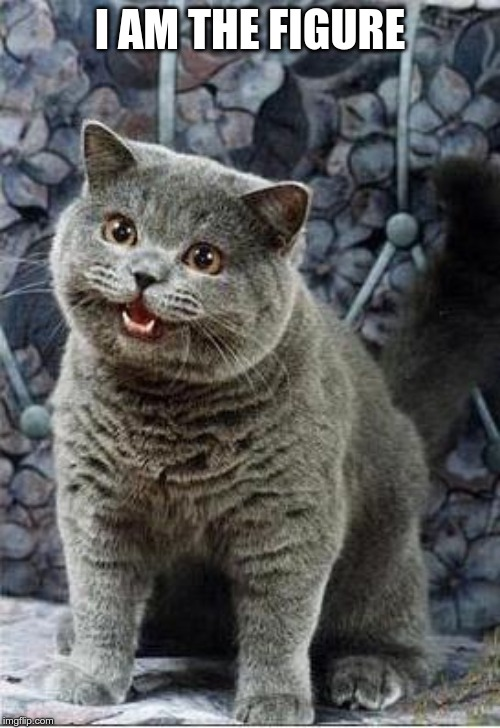
\includegraphics[scale=0.3]{images/figure_filler.jpg}
	\caption[Flowchart of initial model building and automated pipeline steps]{Flowchart of initial model building and automated pipeline steps. Letters indicate the associate steps discussed in the main text.} \label{fig-4-1}
\end{figure}

%%%%%%%%%%%%%%%%%%%%%%
%% Figure 2 website screenshot
%%%%%%%%%%%%%%%%%%%%%%

\begin{figure}
	\centering
		%\includegraphics[scale=0.4]{images/figure_4-2_website_screenshot.png}
		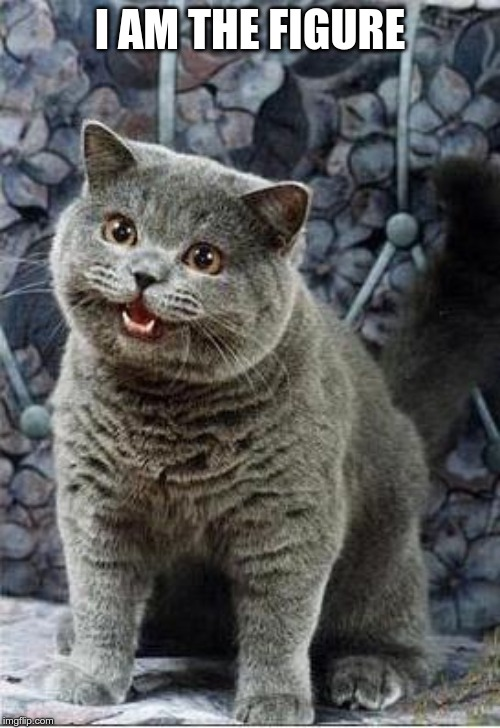
\includegraphics[scale=0.3]{images/figure_filler.jpg}
	\caption[Screenshot of the forecast presentation website]{Screenshot of the forecast presentation website. Shown is the forecast for the leaf out of \textit{Acer saccharinum} in Spring, 2019, issued on Feburary 21, 2019. The maps represent the predicted date of leaf out (A), the anomaly compared to prior years (B), and the 95\% confidence interval (C). In the upper right is the interface for selecting different species, phenophases, or forecast issue dates via drop down menus (D).} \label{fig-4-2}
\end{figure}

%%%%%%%%%%%%%%%%%%%%%%
%% Figure 3 population peak errors
%%%%%%%%%%%%%%%%%%%%%%
\begin{figure}
	\centering
		%\includegraphics[scale=0.6]{images/figure_4-3_map_figure.png}
		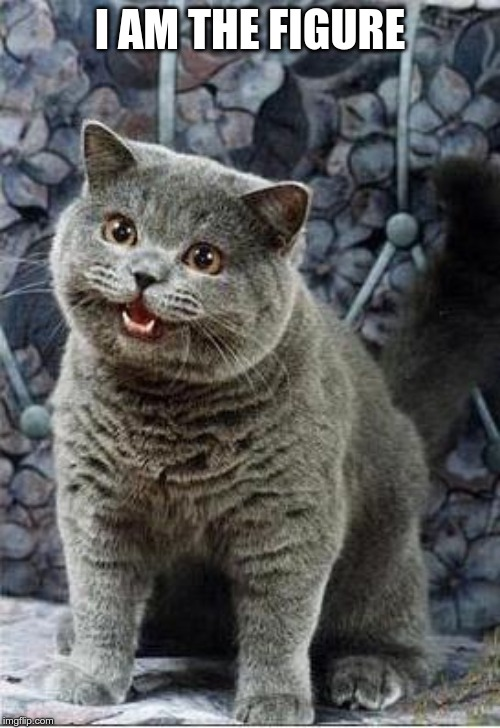
\includegraphics[scale=0.3]{images/figure_filler.jpg}
	\caption[Locations of phenological events which have occurred in 2019]{Locations of phenological events which have occurred in 2019. Events between Jan. 1, 2019 and May 5, 2019 obtained from the USA National Phenology Network (blue circles), and all sampling locations in the same dataset (red points). Four individual plants are highlighted, where the solid line indicates the predicted event date as well as 95\% confidence interval for a specified forecast issue date, and the dashed line indicates the observed event date. The x-axis corresponds to the date a forecast was issued, while the y-axis is the date flowering or budburst was predicted to occur. For example: on Jan. 1, 2019 the \textit{P. tremuloides} plant was forecasted to flower sometime between March, 29 and April, 24 (solid lines), while the actual flowering date was March 18 (dashed line).} \label{fig-4-3}
\end{figure}

%%%%%%%%%%%%%%%%%%%%%%
%% Figure 4 Metric timeseries (RMSE & SD)
%%%%%%%%%%%%%%%%%%%%%%
\begin{figure}
	\centering
		%\includegraphics[scale=0.4]{images/figure_4-4_metric_timeseries.png}
		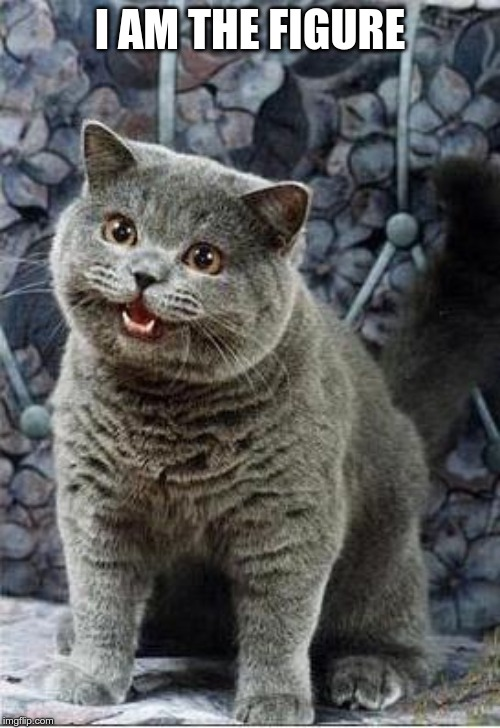
\includegraphics[scale=0.3]{images/figure_filler.jpg}
	\caption[The root mean square error and the average uncertainty of forecasts]{The root mean square error and the average uncertainty of forecasts. Forecasts were issued between Dec. 2, 2018 and May 5, 2019 for 1581 phenological events representing 65 species. } \label{fig-4-4}
\end{figure}

%%%%%%%%%%%%%%%%%%%%%%
%% Figure 5 Error timeseries (MAE Boxplots)
%%%%%%%%%%%%%%%%%%%%%%
\begin{figure}
	\centering
		%\includegraphics[scale=0.3]{images/figure_4-5_error_timeseries.png}
		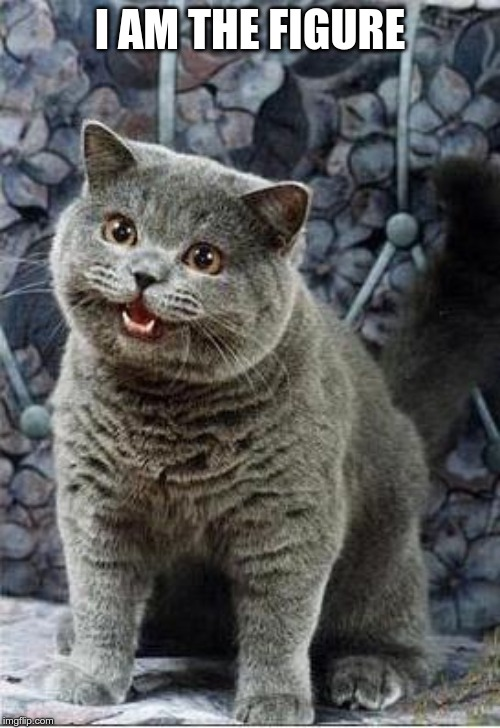
\includegraphics[scale=0.3]{images/figure_filler.jpg}
	\caption[Distribution of absolute errors]{Distribution of absolute errors. The errors (prediction - observed) are for 1581 phenological events for 11 selected issue dates. Labels indicate the mean absolute error (MAE).} \label{fig-4-5}
\end{figure}
\chapter{CONCLUSION} \label{conclusion}

For the validation of citizen science source phenologcial data our results suggest that both LTER and USA-NPN data provide valuable information on plant phenology. Models built using both data sources yield effective predictions for phenological events, but parameter estimates from the two data sources differ and models from each source best predict that data source's phenology events. The primary difference in the datasets is spatial scale, but due to trade-offs in data collection efforts, the larger scale USA-NPN data have shorter time-series, less site fidelity and other differences from the intensively collected LTER data (Table \ref{table-2-3}). These differences can be strengths or potential limitations. Observers sampling opportunistically allows the USA-NPN dataset to have a large spatial scale, but also leads to low site fidelity, which limits the ability to measure long-term trends at local scales \citep{gerst2016}. Tracking long-term trends is the major strength of LTER data, but having a relatively small species pool limits their use in species-level predictive modeling. Due to these differences, the best data source for making predictions depends on the scale at which the predictions are being made. Identifying the most effective data sources for different types and scales of analysis is a useful first step, but the ultimate solution to working with diverse data types is to focus on integrating all types of data into analyses and forecasts \citep{hanks2018, melaas2016}. Our results suggest that methods that can learn from the intensive information available in LTER data in regions where they are available, and simultaneously use large-scale data to capture spatial variation in phenological requirements will help improve our ability to understand and predict phenology. 

In validating the phenological estimators I have used a precise flowering dataset to confirm that naively using the first flowering observation is biased, and estimates using the mean flowering reliable for estimating flowering peak. I have also shown how the recently introduced Weibull method can produce reliable estimates given an adequate sample size. The Logistic and GAM methods can be useful with large datasets having low amounts of flowering presence, and future collection efforts should emphasize absence observations for this reason. Additionally, estimating transition dates of individual plants is best done with the Midway method using a 7 day restriction, and the Weibull method if the restriction results in a low number of final samples. These estimators are needed for translating status-based phenological data into distinct transition dates used to track and forecast changing seasonal patterns.

In conclusion, using recent advances in open source software and large-scale open data collection we have implemented an automated high resolution, continental scale, species-level phenology forecast system. Implementing a system of this scale was made possible by a new phenology data stream and new computational tools that facilitate large scale analysis with limited computing and human resources. Most recent research papers describing ecological forecast systems focus on only the modelling aspect \citep{chen2011, carrillo2018, vandoren2018}, and studies outlining implementation methods and best practices are lacking (but see \cite{white2018, welch2019}). Making a forecast system operational is key to producing applied tools, and requires a significant investment in time and other resources for data logistics and pipeline development. Major challenges here included the automated processing of large meteorological datasets, efficient application of hundreds of phenological models, and stable, consistently updated, and easy to understand dissemination of forecasts. By discussing our approach to automated forecasting on data-intensive questions, and making our code publicly available, we hope to provide guidance for others developing ecological forecasting systems. While many areas for improvement remain for this system, including improved phenology models and more user friendly dissemination of forecasts, this system provides a fully automated actionable forecasts on large scale phenology.
%\include{tex/chapter6}  %These chapters are not included in the template
%\include{tex/chapter7}

%-----------------------------------------------------------------------%

% Use the appropriate file depending upon the number of appendices you have


% The Editorial Office Requirements for the Table of Contents cause a significant problem
%in Latex if there is only one Appendix. The Appendix is no longer labeled "A" in the TOC
%but has the word "APPENDIX" placed in front of the title of the Appendix. This can be done
%without issue IF nothing needs to be numbered by LaTeX in the Appendix. Unfortunately, most of the time
%something needs to be numbered in that single Appendix. For this reason we have included the IFTHENELSE switch
%found in this document and at the beginning of AppendixA. We assume that if you have any appendices, that you have more than one. However, you DO only have one appendix DO NOT USE THIS FILE!!!!!!!!!!!!!!!!!!!!!!!
%
% OneSingleAppendix.tex has all the settings needed to adjust for a single appendix
% you will have a major problem with your TOC if you use this file with a single appendix!!!!!

%
% Comment (or delete) all of the \input{AppendixB} commands except those you are using.
%Then open the AppendixA.tex file and continue there.

%you can add/substract individual appendices through by using the /include{appendix'X'}
% and creating/deleting the appropriate files
\appendix %
%\clearpage%


\addtocontents{toc}{\protect\addvspace{10pt}\protect\noindent \protect APPENDIX\par}

% % % % % % % If you have a single appendix, you should be using appendix1.tex
% % % % % % % NOT this file

\chapter{THIS IS THE FIRST APPENDIX}

Lorem ipsum dolor sit amet, consectetuer adipiscing elit. Maecenas
eget magna. Aenean et lorem. Ut dignissim neque at nisi. In hac
habitasse platea dictumst. In porta ornare eros. Nunc eu ante. In
non est vehicula tellus cursus suscipit. Proin sed libero. Sed risus
enim, eleifend in, pellentesque ac, nonummy quis, nulla. Phasellus
imperdiet libero nec massa. Ut sapien libero, adipiscing eu,
volutpat porttitor, ultricies eget, nisi. Sed odio. Suspendisse
potenti. Duis dolor augue, viverra id, porta in, dignissim id, nisl.
Vivamus blandit cursus eros. Maecenas sit amet urna sit amet orci
nonummy pharetra.

Praesent cursus nibh et mauris. In aliquam felis sit amet ligula.
Nulla faucibus nisl eget nisl. Aliquam tincidunt. Mauris eget elit
sed massa luctus posuere. Pellentesque suscipit. In odio urna,
semper ut, convallis ut, porta et, nibh. Nulla sodales metus nec
velit posuere gravida. Cras tristique. Etiam urna risus, accumsan
ut, placerat sed, iaculis id, est.

Nullam mi. Pellentesque habitant morbi tristique senectus et netus
et malesuada fames ac turpis egestas. Duis vitae metus in massa
hendrerit rhoncus. Fusce tortor justo, laoreet eu, facilisis at,
gravida et, felis. Donec imperdiet mollis erat. Integer tempus nulla
ac lorem. Fusce porttitor. Aenean quis arcu. Morbi consectetuer, leo
eu mollis elementum, urna massa malesuada risus, euismod tempor
lorem elit ut mauris. Cras elit orci, facilisis ac, mattis iaculis,
cursus ac, augue. Donec eget nisl. Pellentesque fermentum sodales
nibh. Vivamus non risus. Donec est libero, tincidunt sit amet,
pretium vitae, blandit sed, tellus. Nunc diam risus, interdum sed,
laoreet quis, varius ac, turpis. In et purus eget nibh vehicula
rhoncus. Aenean et neque. Praesent nisl nisi, tempus quis, nonummy
ac, auctor a, neque. Suspendisse et metus. Suspendisse non metus eu
mauris auctor sagittis.
 %
\chapter{AN EXAMPLE OF A HALF TITLE PAGE}%
\label{appendixB}

\clearpage %remove this command if your appendix doesn't start with a landscaped page!!!!!
\thispagestyle{plain}
\begin{landscape}
\begin{figure}

  \begin{center}
    \includegraphics[width=6in]{images/LaTeX2e_logo.eps}
    \caption{\LaTeX 2\ensuremath{\epsilon.} logo}\label{biglogo}
  \end{center}
\end{figure}
\end{landscape}


This is how a section should look if the first page is a landscape page.
Lorem ipsum dolor sit amet, consectetuer adipiscing elit. Ut sit
amet nulla. Integer mauris turpis, dapibus ac, auctor non, vehicula
sit amet, magna. Suspendisse eu tellus. Etiam porta. Donec magna.
Donec ut dui. In hac habitasse platea dictumst. Nullam suscipit, mi
at adipiscing commodo, lorem erat scelerisque erat, non pulvinar leo
mi eu metus. Phasellus id felis. Sed quam purus, molestie quis,
ultrices nec, dictum at, magna. Proin viverra viverra ante.

Maecenas sagittis magna quis ligula. Duis vestibulum mi a felis.
Aenean accumsan mattis massa. Nullam lacus sem, consectetuer non,
condimentum sit amet, pharetra ac, odio. Morbi nisi magna, tincidunt
sed, placerat nec, tincidunt id, lectus. Donec ac dui non mauris
vulputate aliquam. Nullam scelerisque congue pede. Integer ipsum.
Vestibulum auctor. Suspendisse eget leo id libero cursus dictum. Sed
malesuada. Aliquam imperdiet. Donec dui metus, porta eu, aliquet
vel, vulputate vitae, lacus.

Nulla quis purus id turpis luctus feugiat. Fusce feugiat. Proin
felis. Morbi elit est, fermentum in, tincidunt vitae, convallis vel,
orci. Vestibulum justo. Suspendisse non nisl. Pellentesque pretium
adipiscing elit. Phasellus fermentum consequat augue. Sed pede nisl,
fermentum vel, vulputate id, sollicitudin sed, ligula. Cras
suscipit, quam et euismod sagittis, nisl felis gravida felis, quis
pulvinar purus est vel pede. Suspendisse mattis est ac nunc.
Curabitur rutrum, turpis sit amet commodo tempus, metus lorem
commodo lectus, eget fringilla justo nisi et purus. Ut quam sapien,
vehicula quis, rhoncus non, sagittis nec, risus.

Donec eget augue ac lacus adipiscing porta. Maecenas pede. Vivamus
molestie. Duis condimentum ligula auctor pede. Nullam ullamcorper
rhoncus erat. Ut ornare interdum urna. Suspendisse potenti.
Curabitur mattis mauris nec risus. Aenean iaculis turpis eu tortor.
Donec nec ante non mauris pellentesque fringilla.

Phasellus vitae dui id orci sodales cursus. Curabitur sed nulla quis
mauris tincidunt iaculis. Vivamus semper semper orci. Phasellus
suscipit ante vitae leo. Sed arcu ipsum, condimentum id, luctus in,
sodales eu, magna. In dictum, arcu quis pharetra vestibulum, ante
enim placerat lacus, vitae placerat est leo vitae elit. Pellentesque
bibendum enim vulputate eros. Nunc laoreet. Pellentesque habitant
morbi tristique senectus et netus et malesuada fames ac turpis
egestas. Praesent purus odio, euismod sit amet, aliquam a, volutpat
in, augue. Phasellus id massa. Suspendisse suscipit ligula pharetra
dolor. Pellentesque vel pede.

Aliquam pharetra est sit amet magna. Aliquam varius. Donec eu lectus
et nisl iaculis porttitor. Morbi mattis, mauris sed luctus
hendrerit, nulla velit molestie dolor, ac volutpat urna augue vel
quam. Maecenas pellentesque libero et massa. Integer vestibulum,
lacus at mattis euismod, nisl arcu commodo lectus, ut euismod dolor
ligula sit amet libero. Nam in ligula sit amet ante eleifend
aliquet. Phasellus feugiat erat at nulla. Proin in lectus. Proin
laoreet leo laoreet leo congue lacinia. Quisque non diam sit amet
enim ultrices commodo. Praesent fermentum lectus sed ligula. Integer
pulvinar accumsan pede. Quisque molestie ligula eget odio.
Vestibulum ante ipsum primis in faucibus orci luctus et ultrices
posuere cubilia Curae;
 %
\chapter{SUPPLEMENTARY MATERIAL FOR CHAPTER 4}

\section{Description of the Phenology Model Weighting}\label{appendix-a}

We used a weighted ensemble of the four models for each species and phenophase. The weights for each model within the ensemble were derived via stacking as described in \cite{dormann2018}. The steps for calculating weights are as followed:

\begin{enumerate}
    \item Subset the phenology data into random training/testing sets.
    \item Fit each core model on the training set.
    \item Make predictions on the testing set.
    \item Find the weights which minimize RMSE of the testing set.
    \item Repeat 1-4 for 100 iterations.
    \item Take the average weight for each model from all iterations as the final weight used in the ensemble. These will sum to 1.
    \item Fit the core models a final time on the full dataset. Parameters derived from this final iterations will be used to make predictions, which are then used in the final weighted average. 
\end{enumerate}

The four phenology models are applied to each of the five members of the climate ensemble, with a final predicted value, $\widehat{DOY}_{forecast}$, derived as:

$$\widehat{DOY}_{forecast} = \frac{1}{5}\sum_{n=1}^{5}\sum_{i=1}^{4}w_{i}\widehat{DOY}_{n,i}$$

Where $n$ is the climate ensemble member, $i$ is the phenology model, $w$ is the phenology model weight, and $\widehat{DOY}$ the estimated Julian day. 

Uncertainty is the 95\% confidience interval of the estimates from the five climate ensembles:

$$2 * \sqrt{\frac{1}{5}\sum_{n=1}^{5}(\widehat{DOY}_{n} - \widehat{DOY}_{forecast})^{2}}$$


\section{Description of the Climate Downscaling Model}

The Climate Forecast System Version 2 (CFSv2) is a coupled atmosphere-ocean-land global circulation model maintained by the National Oceanic and Atmospheric Administration (NOAA)[@saha2014]. The model tracks over 1000 global state variables of varying resolution and forecast length, such as ocean temperature and heights of pressure bands. Here we use the 2-meter temperature variable, which has a 6-hour timestep and a spatial resolution of 0.25 degrees latitude/longitude. The forecast is updated every 6 hours with the latest initial conditions and projected out 9 months. 

The CFSv2 also has a reanalysis available. A climate reanalysis is a run of the full model over a prior time period with constant assimilation of known conditions. In practice this allows for analysis of state variables which are not able to be measured (such as the 500mb height over the arctic in winter). Here it allows us to build a downscaling model using the CFSv2 model’s best estimate of past conditions of land surface temperature. These past conditions are regressed against finer grained “known” conditions from a different gridded dataset on a per pixel basis. We used the 2-m temperature output from the reanalysis from 1995-2015 as well as 4km daily mean temperature from the PRISM dataset \citep{prismdata} to build a downscaling model using asynchronous regression (Figure \ref{fig-4-1}). The model and theory are described in \cite{stoner2013} and references therein. The CFSv2 data is first interpolated from the original 0.25 degree grid to a 4km grid using distance weighted sampling, then the following method is applied to each 4km pixel and calendar month.

\begin{enumerate}
    \item Collect all daily mean temperature observations from 21 years of data from both the CFSv2 reanalysis and the PRISM dataset. This provides 588 - 641 points representing daily temperature for a single pixel and calendar month.
    \item In addition to the data from each calendar month, also include data for the 14 days prior and 14 days following the calendar month, adding an addition 588 data points (21*(14+14)). This helps account for future novel conditions.
    \item Order each dataset by their rank, such that the lowest value from the PRISM dataset is matched to the lowest value from the CFSv2 reanalysis.
    \item Fit a linear regression model.
\end{enumerate}

The two parameters from the regression model are saved in a netCFD file which can later be referenced by location and calendar month (Figure \ref{fig-4-1}, H). This downscaling model, at the scale of the continental U.S.A., is used to downscale the most recent CFSv2 forecasts to a 4km resolution during the automated steps. 

%%%%%%%%%%%%%%%%%
%% Table C1 - Species and their associated phenophases used in the forecast system
%%%%%%%%%%%%%%%%%
\newpage

\section{Supplementary Tables}

\begin{table}
    \caption[Species and their associated phenophases used in the forecast system]{Species and their associated phenophases used in the forecast system. Note not all species have forecasts for all phenophases due to data availability. A * indicates a contributed model which was not built using USA-NPN data.}
    \label{table-c-1}
\begin{tabularx}{\textwidth}{p{0.5cm}XXXXX}
\hline
& Species & Budburst & Fall Colors & Flowers & Ripe Fruits\\
\hline

1 & Acacia greggii &  &  & $\checkmark$ &  \\ 
2 & Acer circinatum & $\checkmark$ &  & $\checkmark$ &  \\ 
3 & Acer macrophyllum & $\checkmark$ &  & $\checkmark$ &  \\ 
4 & Acer negundo & $\checkmark$ & $\checkmark$ & $\checkmark$ &  \\ 
5 & Acer pensylvanicum & $\checkmark$ & $\checkmark$ & $\checkmark$ &  \\ 
6 & Acer rubrum & $\checkmark$ & $\checkmark$ & $\checkmark$ &  \\ 
7 & Acer saccharinum & $\checkmark$ & $\checkmark$ & $\checkmark$ &  \\ 
8 & Acer saccharum & $\checkmark$ & $\checkmark$ & $\checkmark$ &  \\ 
9 & Aesculus californica & $\checkmark$ & $\checkmark$ & $\checkmark$ &  \\ 
10 & Alnus incana & $\checkmark$ & $\checkmark$ & $\checkmark$ &  \\ 
11 & Alnus rubra & $\checkmark$ & $\checkmark$ &  &  \\ 
12 & Amelanchier alnifolia & $\checkmark$ & $\checkmark$ & $\checkmark$ &  \\ 
13 & Artemisia tridentata &  &  & $\checkmark$ &  \\ 
14 & Berberis aquifolium* &  &  & $\checkmark$ & $\checkmark$ \\ 
15 & Betula alleghaniensis & $\checkmark$ & $\checkmark$ & $\checkmark$ &  \\ 
16 & Betula lenta & $\checkmark$ & $\checkmark$ & $\checkmark$ &  \\ 
17 & Betula nigra & $\checkmark$ &  & $\checkmark$ &  \\ 
18 & Betula papyrifera & $\checkmark$ & $\checkmark$ & $\checkmark$ &  \\ 
19 & Carpinus caroliniana & $\checkmark$ & $\checkmark$ & $\checkmark$ &  \\ 
20 & Carya glabra & $\checkmark$ & $\checkmark$ & $\checkmark$ &  \\ 

\hline
\end{tabularx}
\end{table}

% Table C-1 continued, page 2/4

\begin{table}
\begin{tabularx}{\textwidth}{p{0.5cm}XXXXX}
\multicolumn{3}{l}{Table \ref{table-c-1}. Continued}\\
\hline
& Species & Budburst & Fall Colors & Flowers & Ripe Fruits\\
\hline
21 & Celtis occidentalis & $\checkmark$ &  &  &  \\ 
22 & Cephalanthus occidentalis & $\checkmark$ &  & $\checkmark$ &  \\ 
23 & Cercis canadensis & $\checkmark$ & $\checkmark$ & $\checkmark$ &  \\ 
24 & Chilopsis linearis &  &  & $\checkmark$ &  \\ 
25 & Clintonia borealis &  &  & $\checkmark$ &  \\ 
26 & Cornus florida & $\checkmark$ & $\checkmark$ & $\checkmark$ &  \\ 
27 & Cornus racemosa & $\checkmark$ &  &  &  \\ 
28 & Cornus sericea & $\checkmark$ & $\checkmark$ & $\checkmark$ &  \\ 
29 & Corylus cornuta* &  &  & $\checkmark$ & $\checkmark$ \\ 
30 & Diospyros virginiana & $\checkmark$ &  &  &  \\ 
31 & Fagus grandifolia & $\checkmark$ & $\checkmark$ & $\checkmark$ &  \\ 
32 & Fouquieria splendens &  &  & $\checkmark$ &  \\ 
33 & Fraxinus americana & $\checkmark$ & $\checkmark$ & $\checkmark$ &  \\ 
34 & Fraxinus pennsylvanica & $\checkmark$ & $\checkmark$ & $\checkmark$ &  \\ 
35 & Gaultheria shallon* &  &  & $\checkmark$ & $\checkmark$ \\ 
36 & Ginkgo biloba & $\checkmark$ & $\checkmark$ & $\checkmark$ &  \\ 
37 & Gleditsia triacanthos & $\checkmark$ & $\checkmark$ & $\checkmark$ &  \\ 
38 & Hamamelis virginiana & $\checkmark$ & $\checkmark$ & $\checkmark$ &  \\ 
39 & Ilex verticillata & $\checkmark$ &  & $\checkmark$ &  \\ 
40 & Juglans nigra & $\checkmark$ & $\checkmark$ & $\checkmark$ &  \\ 


\hline
\end{tabularx}
\end{table}

% Table C-1 continued, page 3/4

\begin{table}
\begin{tabularx}{\textwidth}{p{0.5cm}XXXXX}
\multicolumn{3}{l}{Table \ref{table-c-1}. Continued}\\
\hline
& Species & Budburst & Fall Colors & Flowers & Ripe Fruits\\
\hline
41 & Liquidambar styraciflua & $\checkmark$ & $\checkmark$ & $\checkmark$ &  \\ 
42 & Liriodendron tulipifera & $\checkmark$ & $\checkmark$ & $\checkmark$ &  \\ 
43 & Magnolia grandiflora & $\checkmark$ &  & $\checkmark$ &  \\ 
44 & Maianthemum canadense &  &  & $\checkmark$ &  \\ 
45 & Nyssa sylvatica & $\checkmark$ &  & $\checkmark$ &  \\ 
46 & Ostrya virginiana & $\checkmark$ &  & $\checkmark$ &  \\ 
47 & Oxydendrum arboreum & $\checkmark$ & $\checkmark$ & $\checkmark$ &  \\ 
48 & Platanthera praeclara & $\checkmark$ &  & $\checkmark$ &  \\ 
49 & Platanus racemosa & $\checkmark$ &  & $\checkmark$ &  \\ 
50 & Populus deltoides & $\checkmark$ & $\checkmark$ & $\checkmark$ &  \\ 
51 & Populus fremontii & $\checkmark$ & $\checkmark$ & $\checkmark$ &  \\ 
52 & Populus tremuloides & $\checkmark$ & $\checkmark$ & $\checkmark$ &  \\ 
53 & Prunus americana & $\checkmark$ &  & $\checkmark$ &  \\ 
54 & Prunus serotina & $\checkmark$ & $\checkmark$ & $\checkmark$ &  \\ 
55 & Prunus virginiana & $\checkmark$ & $\checkmark$ & $\checkmark$ &  \\ 
56 & Quercus agrifolia & $\checkmark$ &  & $\checkmark$ &  \\ 
57 & Quercus alba & $\checkmark$ & $\checkmark$ & $\checkmark$ &  \\ 
58 & Quercus douglasii & $\checkmark$ & $\checkmark$ & $\checkmark$ &  \\ 
59 & Quercus gambelii & $\checkmark$ & $\checkmark$ &  &  \\ 
60 & Quercus laurifolia & $\checkmark$ &  &  &  \\ 



\hline
\end{tabularx}
\end{table}

% Table C-1 continued, page 4/4

\begin{table}
\begin{tabularx}{\textwidth}{p{0.5cm}XXXXX}
\multicolumn{3}{l}{Table \ref{table-c-1}. Continued}\\
\hline
& Species & Budburst & Fall Colors & Flowers & Ripe Fruits\\
\hline
61 & Quercus lobata & $\checkmark$ & $\checkmark$ & $\checkmark$ &  \\ 
62 & Quercus macrocarpa & $\checkmark$ & $\checkmark$ & $\checkmark$ &  \\ 
63 & Quercus palustris & $\checkmark$ & $\checkmark$ & $\checkmark$ &  \\ 
64 & Quercus rubra & $\checkmark$ & $\checkmark$ & $\checkmark$ &  \\ 
65 & Quercus velutina & $\checkmark$ & $\checkmark$ & $\checkmark$ &  \\ 
66 & Quercus virginiana & $\checkmark$ &  & $\checkmark$ &  \\ 
67 & Rhododendron macrophyllum & $\checkmark$ &  & $\checkmark$ &  \\ 
68 & Robinia pseudoacacia & $\checkmark$ & $\checkmark$ & $\checkmark$ &  \\ 
69 & Salix hookeriana & $\checkmark$ & $\checkmark$ & $\checkmark$ &  \\ 
70 & Salix lasiolepis & $\checkmark$ &  & $\checkmark$ &  \\ 
71 & Sassafras albidum & $\checkmark$ & $\checkmark$ & $\checkmark$ &  \\ 
72 & Sorbus americana & $\checkmark$ & $\checkmark$ & $\checkmark$ &  \\ 
73 & Tilia americana & $\checkmark$ & $\checkmark$ & $\checkmark$ &  \\ 
74 & Ulmus americana & $\checkmark$ & $\checkmark$ & $\checkmark$ &  \\ 
75 & Umbellularia californica & $\checkmark$ &  & $\checkmark$ &  \\ 
76 & Vaccinium corymbosum & $\checkmark$ & $\checkmark$ & $\checkmark$ &  \\ 
77 & Vaccinium membranaceum* &  &  & $\checkmark$ & $\checkmark$ \\ 
78 & Yucca brevifolia &  &  & $\checkmark$ &  \\ 
 & **Total** & **67** & **47** & **72** & **4** \\ 


\hline
\end{tabularx}
\end{table}


%%%%%%%%%%%%%%%%%
%% Table C2 - Species and their associated phenophases evaluated from the 2019 season
%%%%%%%%%%%%%%%%%
\newpage

\begin{table}
    \caption[Species and their associated phenophases evaluated from the 2019 season]{Species and their associated phenophases evaluated from the 2019 season. Numbers indicate the total observations for the species and phenophase, with the mean Julian day in parentheses. Data are from the USA National Phenology Network from Jan. 1, 2019 - May 8, 2019.}
    \label{table-c-2}
\begin{tabularx}{\textwidth}{p{0.5cm}XXXXX}
\hline
 & Species & Budburst & Fall Colors & Flowers \\ 
\hline

1 & Acer circinatum & 38 (93.1) &  & 25 (112.4) \\ 
2 & Acer macrophyllum & 10 (90.6) &  & 6 (94.7) \\ 
3 & Acer negundo & 14 (98.7) &  & 13 (86.1) \\ 
4 & Acer pensylvanicum & 6 (93.8) &  & 2 (91) \\ 
5 & Acer rubrum & 177 (93) &  & 152 (86.1) \\ 
6 & Acer saccharinum & 10 (107) &  & 6 (99.3) \\ 
7 & Acer saccharum & 56 (105.5) &  & 30 (109.8) \\ 
8 & Aesculus californica & 3 (46.3) & 2 (115) & 5 (118.2) \\ 
9 & Alnus incana & 1 (107) &  &  \\ 
10 & Alnus rubra & 6 (85.2) &  &  \\ 
11 & Amelanchier alnifolia & 1 (83) &  &  \\ 
12 & Betula alleghaniensis & 7 (114.3) &  & 4 (122.5) \\ 
13 & Betula lenta & 28 (99.2) &  & 11 (106.5) \\ 
14 & Betula nigra & 1 (104) &  & 1 (87) \\ 
15 & Betula papyrifera & 5 (112) &  & 6 (113.8) \\ 
16 & Carpinus caroliniana & 28 (82.1) &  & 20 (80) \\ 
17 & Carya glabra & 6 (77.2) &  & 5 (112.8) \\ 
18 & Celtis occidentalis & 4 (105.5) &  &  \\ 
19 & Cephalanthus occidentalis & 9 (102) &  &  \\ 
20 & Cercis canadensis & 22 (94.1) &  & 24 (93) \\ 
21 & Chilopsis linearis &  &  & 4 (119) \\ 
22 & Cornus florida & 69 (89.7) &  & 56 (101.8) \\ 
23 & Cornus racemosa & 6 (102.5) &  &  \\ 
24 & Cornus sericea & 9 (103.4) &  &  \\ 
25 & Corylus cornuta &  &  & 4 (57.8) \\ 

\hline
\end{tabularx}
\end{table}


% Table C-2 continued, page 2/3

\begin{table}
\begin{tabularx}{\textwidth}{p{0.5cm}XXXXX}
\multicolumn{3}{l}{Table \ref{table-c-2}. Continued}\\
\hline
& Species & Budburst & Fall Colors & Flowers\\
\hline

26 & Diospyros virginiana & 1 (124) &  &  \\ 
27 & Fagus grandifolia & 45 (100.9) &  & 10 (114.2) \\ 
28 & Fouquieria splendens &  &  & 9 (97.7) \\ 
29 & Fraxinus americana & 3 (109.7) &  &  \\ 
30 & Fraxinus pennsylvanica & 2 (112.5) &  &  \\ 
31 & Ginkgo biloba & 5 (108.6) &  & 1 (111) \\ 
32 & Hamamelis virginiana & 23 (104.3) &  &  \\ 
33 & Ilex verticillata & 3 (115.3) &  &  \\ 
34 & Juglans nigra & 5 (106.6) &  & 4 (107.2) \\ 
35 & Liquidambar styraciflua & 18 (75.2) &  & 13 (89) \\ 
36 & Liriodendron tulipifera & 41 (88.4) &  & 14 (86.2) \\ 
37 & Magnolia grandiflora & 5 (85.8) &  & 7 (104.7) \\ 
38 & Nyssa sylvatica & 17 (99) &  & 1 (76) \\ 
39 & Ostrya virginiana & 4 (91.5) &  &  \\ 
40 & Oxydendrum arboreum & 8 (98.6) &  & 1 (76) \\ 
41 & Platanus racemosa & 5 (22) &  & 3 (46) \\ 
42 & Populus deltoides & 8 (111.8) &  & 5 (110.6) \\ 
43 & Populus fremontii & 2 (102) &  &  \\ 
44 & Populus tremuloides & 10 (113) &  & 11 (97.6) \\ 
45 & Prunus americana & 1 (111) &  & 1 (112) \\ 

\hline
\end{tabularx}
\end{table}


% Table C-2 continued, page 3/3

\begin{table}
\begin{tabularx}{\textwidth}{p{0.5cm}XXXXX}
\multicolumn{3}{l}{Table \ref{table-c-2}. Continued}\\
\hline
& Species & Budburst & Fall Colors & Flowers\\
\hline

46 & Prunus serotina & 30 (84.1) &  & 10 (70.7) \\ 
47 & Prunus virginiana & 6 (95.2) &  & 1 (107) \\ 
48 & Quercus agrifolia & 32 (68.7) &  & 12 (83.2) \\ 
49 & Quercus alba & 32 (100) &  & 14 (112.7) \\ 
50 & Quercus douglasii & 4 (81.8) &  & 3 (108) \\ 
51 & Quercus gambelii & 16 (114.2) &  &  \\ 
52 & Quercus laurifolia & 9 (50.4) &  &  \\ 
53 & Quercus lobata & 14 (63.9) &  & 4 (81) \\ 
54 & Quercus macrocarpa & 23 (108.5) &  & 10 (120.5) \\ 
55 & Quercus palustris & 4 (103) &  & 2 (113) \\ 
56 & Quercus rubra & 47 (105.8) &  & 24 (112.9) \\ 
57 & Quercus velutina & 4 (102.8) &  & 3 (106) \\ 
58 & Quercus virginiana & 10 (58) &  & 11 (66.5) \\ 
59 & Sassafras albidum & 6 (108) &  & 8 (108) \\ 
60 & Sorbus americana & 2 (124) &  &  \\ 
61 & Tilia americana & 7 (101.9) &  &  \\ 
62 & Ulmus americana & 8 (80.8) &  & 2 (42) \\ 
63 & Umbellularia californica & 5 (98.8) &  & 5 (54.6) \\ 
64 & Vaccinium corymbosum & 10 (81.1) &  & 15 (90.4) \\ 
65 & Yucca brevifolia &  &  & 10 (76.4) \\ 
 & Total & 991 (93.8) & 2 (115) & 588 (94.8) \\ 
 
\hline
\end{tabularx}
\end{table} %
%\chapter{SUPPLEMENTARY MATERIAL FOR CHAPTER 4}

\section{Description of the Phenology Model Weighting}\label{appendix-a}

We used a weighted ensemble of the four models for each species and phenophase. The weights for each model within the ensemble were derived via stacking as described in \cite{dormann2018}. The steps for calculating weights are as followed:

\begin{enumerate}
    \item Subset the phenology data into random training/testing sets.
    \item Fit each core model on the training set.
    \item Make predictions on the testing set.
    \item Find the weights which minimize RMSE of the testing set.
    \item Repeat 1-4 for 100 iterations.
    \item Take the average weight for each model from all iterations as the final weight used in the ensemble. These will sum to 1.
    \item Fit the core models a final time on the full dataset. Parameters derived from this final iterations will be used to make predictions, which are then used in the final weighted average. 
\end{enumerate}

The four phenology models are applied to each of the five members of the climate ensemble, with a final predicted value, $\widehat{DOY}_{forecast}$, derived as:

$$\widehat{DOY}_{forecast} = \frac{1}{5}\sum_{n=1}^{5}\sum_{i=1}^{4}w_{i}\widehat{DOY}_{n,i}$$

Where $n$ is the climate ensemble member, $i$ is the phenology model, $w$ is the phenology model weight, and $\widehat{DOY}$ the estimated Julian day. 

Uncertainty is the 95\% confidience interval of the estimates from the five climate ensembles:

$$2 * \sqrt{\frac{1}{5}\sum_{n=1}^{5}(\widehat{DOY}_{n} - \widehat{DOY}_{forecast})^{2}}$$


\section{Description of the Climate Downscaling Model}

The Climate Forecast System Version 2 (CFSv2) is a coupled atmosphere-ocean-land global circulation model maintained by the National Oceanic and Atmospheric Administration (NOAA)[@saha2014]. The model tracks over 1000 global state variables of varying resolution and forecast length, such as ocean temperature and heights of pressure bands. Here we use the 2-meter temperature variable, which has a 6-hour timestep and a spatial resolution of 0.25 degrees latitude/longitude. The forecast is updated every 6 hours with the latest initial conditions and projected out 9 months. 

The CFSv2 also has a reanalysis available. A climate reanalysis is a run of the full model over a prior time period with constant assimilation of known conditions. In practice this allows for analysis of state variables which are not able to be measured (such as the 500mb height over the arctic in winter). Here it allows us to build a downscaling model using the CFSv2 model’s best estimate of past conditions of land surface temperature. These past conditions are regressed against finer grained “known” conditions from a different gridded dataset on a per pixel basis. We used the 2-m temperature output from the reanalysis from 1995-2015 as well as 4km daily mean temperature from the PRISM dataset \citep{prismdata} to build a downscaling model using asynchronous regression (Figure \ref{fig-4-1}). The model and theory are described in \cite{stoner2013} and references therein. The CFSv2 data is first interpolated from the original 0.25 degree grid to a 4km grid using distance weighted sampling, then the following method is applied to each 4km pixel and calendar month.

\begin{enumerate}
    \item Collect all daily mean temperature observations from 21 years of data from both the CFSv2 reanalysis and the PRISM dataset. This provides 588 - 641 points representing daily temperature for a single pixel and calendar month.
    \item In addition to the data from each calendar month, also include data for the 14 days prior and 14 days following the calendar month, adding an addition 588 data points (21*(14+14)). This helps account for future novel conditions.
    \item Order each dataset by their rank, such that the lowest value from the PRISM dataset is matched to the lowest value from the CFSv2 reanalysis.
    \item Fit a linear regression model.
\end{enumerate}

The two parameters from the regression model are saved in a netCFD file which can later be referenced by location and calendar month (Figure \ref{fig-4-1}, H). This downscaling model, at the scale of the continental U.S.A., is used to downscale the most recent CFSv2 forecasts to a 4km resolution during the automated steps. 

%%%%%%%%%%%%%%%%%
%% Table C1 - Species and their associated phenophases used in the forecast system
%%%%%%%%%%%%%%%%%
\newpage

\section{Supplementary Tables}

\begin{table}
    \caption[Species and their associated phenophases used in the forecast system]{Species and their associated phenophases used in the forecast system. Note not all species have forecasts for all phenophases due to data availability. A * indicates a contributed model which was not built using USA-NPN data.}
    \label{table-c-1}
\begin{tabularx}{\textwidth}{p{0.5cm}XXXXX}
\hline
& Species & Budburst & Fall Colors & Flowers & Ripe Fruits\\
\hline

1 & Acacia greggii &  &  & $\checkmark$ &  \\ 
2 & Acer circinatum & $\checkmark$ &  & $\checkmark$ &  \\ 
3 & Acer macrophyllum & $\checkmark$ &  & $\checkmark$ &  \\ 
4 & Acer negundo & $\checkmark$ & $\checkmark$ & $\checkmark$ &  \\ 
5 & Acer pensylvanicum & $\checkmark$ & $\checkmark$ & $\checkmark$ &  \\ 
6 & Acer rubrum & $\checkmark$ & $\checkmark$ & $\checkmark$ &  \\ 
7 & Acer saccharinum & $\checkmark$ & $\checkmark$ & $\checkmark$ &  \\ 
8 & Acer saccharum & $\checkmark$ & $\checkmark$ & $\checkmark$ &  \\ 
9 & Aesculus californica & $\checkmark$ & $\checkmark$ & $\checkmark$ &  \\ 
10 & Alnus incana & $\checkmark$ & $\checkmark$ & $\checkmark$ &  \\ 
11 & Alnus rubra & $\checkmark$ & $\checkmark$ &  &  \\ 
12 & Amelanchier alnifolia & $\checkmark$ & $\checkmark$ & $\checkmark$ &  \\ 
13 & Artemisia tridentata &  &  & $\checkmark$ &  \\ 
14 & Berberis aquifolium* &  &  & $\checkmark$ & $\checkmark$ \\ 
15 & Betula alleghaniensis & $\checkmark$ & $\checkmark$ & $\checkmark$ &  \\ 
16 & Betula lenta & $\checkmark$ & $\checkmark$ & $\checkmark$ &  \\ 
17 & Betula nigra & $\checkmark$ &  & $\checkmark$ &  \\ 
18 & Betula papyrifera & $\checkmark$ & $\checkmark$ & $\checkmark$ &  \\ 
19 & Carpinus caroliniana & $\checkmark$ & $\checkmark$ & $\checkmark$ &  \\ 
20 & Carya glabra & $\checkmark$ & $\checkmark$ & $\checkmark$ &  \\ 

\hline
\end{tabularx}
\end{table}

% Table C-1 continued, page 2/4

\begin{table}
\begin{tabularx}{\textwidth}{p{0.5cm}XXXXX}
\multicolumn{3}{l}{Table \ref{table-c-1}. Continued}\\
\hline
& Species & Budburst & Fall Colors & Flowers & Ripe Fruits\\
\hline
21 & Celtis occidentalis & $\checkmark$ &  &  &  \\ 
22 & Cephalanthus occidentalis & $\checkmark$ &  & $\checkmark$ &  \\ 
23 & Cercis canadensis & $\checkmark$ & $\checkmark$ & $\checkmark$ &  \\ 
24 & Chilopsis linearis &  &  & $\checkmark$ &  \\ 
25 & Clintonia borealis &  &  & $\checkmark$ &  \\ 
26 & Cornus florida & $\checkmark$ & $\checkmark$ & $\checkmark$ &  \\ 
27 & Cornus racemosa & $\checkmark$ &  &  &  \\ 
28 & Cornus sericea & $\checkmark$ & $\checkmark$ & $\checkmark$ &  \\ 
29 & Corylus cornuta* &  &  & $\checkmark$ & $\checkmark$ \\ 
30 & Diospyros virginiana & $\checkmark$ &  &  &  \\ 
31 & Fagus grandifolia & $\checkmark$ & $\checkmark$ & $\checkmark$ &  \\ 
32 & Fouquieria splendens &  &  & $\checkmark$ &  \\ 
33 & Fraxinus americana & $\checkmark$ & $\checkmark$ & $\checkmark$ &  \\ 
34 & Fraxinus pennsylvanica & $\checkmark$ & $\checkmark$ & $\checkmark$ &  \\ 
35 & Gaultheria shallon* &  &  & $\checkmark$ & $\checkmark$ \\ 
36 & Ginkgo biloba & $\checkmark$ & $\checkmark$ & $\checkmark$ &  \\ 
37 & Gleditsia triacanthos & $\checkmark$ & $\checkmark$ & $\checkmark$ &  \\ 
38 & Hamamelis virginiana & $\checkmark$ & $\checkmark$ & $\checkmark$ &  \\ 
39 & Ilex verticillata & $\checkmark$ &  & $\checkmark$ &  \\ 
40 & Juglans nigra & $\checkmark$ & $\checkmark$ & $\checkmark$ &  \\ 


\hline
\end{tabularx}
\end{table}

% Table C-1 continued, page 3/4

\begin{table}
\begin{tabularx}{\textwidth}{p{0.5cm}XXXXX}
\multicolumn{3}{l}{Table \ref{table-c-1}. Continued}\\
\hline
& Species & Budburst & Fall Colors & Flowers & Ripe Fruits\\
\hline
41 & Liquidambar styraciflua & $\checkmark$ & $\checkmark$ & $\checkmark$ &  \\ 
42 & Liriodendron tulipifera & $\checkmark$ & $\checkmark$ & $\checkmark$ &  \\ 
43 & Magnolia grandiflora & $\checkmark$ &  & $\checkmark$ &  \\ 
44 & Maianthemum canadense &  &  & $\checkmark$ &  \\ 
45 & Nyssa sylvatica & $\checkmark$ &  & $\checkmark$ &  \\ 
46 & Ostrya virginiana & $\checkmark$ &  & $\checkmark$ &  \\ 
47 & Oxydendrum arboreum & $\checkmark$ & $\checkmark$ & $\checkmark$ &  \\ 
48 & Platanthera praeclara & $\checkmark$ &  & $\checkmark$ &  \\ 
49 & Platanus racemosa & $\checkmark$ &  & $\checkmark$ &  \\ 
50 & Populus deltoides & $\checkmark$ & $\checkmark$ & $\checkmark$ &  \\ 
51 & Populus fremontii & $\checkmark$ & $\checkmark$ & $\checkmark$ &  \\ 
52 & Populus tremuloides & $\checkmark$ & $\checkmark$ & $\checkmark$ &  \\ 
53 & Prunus americana & $\checkmark$ &  & $\checkmark$ &  \\ 
54 & Prunus serotina & $\checkmark$ & $\checkmark$ & $\checkmark$ &  \\ 
55 & Prunus virginiana & $\checkmark$ & $\checkmark$ & $\checkmark$ &  \\ 
56 & Quercus agrifolia & $\checkmark$ &  & $\checkmark$ &  \\ 
57 & Quercus alba & $\checkmark$ & $\checkmark$ & $\checkmark$ &  \\ 
58 & Quercus douglasii & $\checkmark$ & $\checkmark$ & $\checkmark$ &  \\ 
59 & Quercus gambelii & $\checkmark$ & $\checkmark$ &  &  \\ 
60 & Quercus laurifolia & $\checkmark$ &  &  &  \\ 



\hline
\end{tabularx}
\end{table}

% Table C-1 continued, page 4/4

\begin{table}
\begin{tabularx}{\textwidth}{p{0.5cm}XXXXX}
\multicolumn{3}{l}{Table \ref{table-c-1}. Continued}\\
\hline
& Species & Budburst & Fall Colors & Flowers & Ripe Fruits\\
\hline
61 & Quercus lobata & $\checkmark$ & $\checkmark$ & $\checkmark$ &  \\ 
62 & Quercus macrocarpa & $\checkmark$ & $\checkmark$ & $\checkmark$ &  \\ 
63 & Quercus palustris & $\checkmark$ & $\checkmark$ & $\checkmark$ &  \\ 
64 & Quercus rubra & $\checkmark$ & $\checkmark$ & $\checkmark$ &  \\ 
65 & Quercus velutina & $\checkmark$ & $\checkmark$ & $\checkmark$ &  \\ 
66 & Quercus virginiana & $\checkmark$ &  & $\checkmark$ &  \\ 
67 & Rhododendron macrophyllum & $\checkmark$ &  & $\checkmark$ &  \\ 
68 & Robinia pseudoacacia & $\checkmark$ & $\checkmark$ & $\checkmark$ &  \\ 
69 & Salix hookeriana & $\checkmark$ & $\checkmark$ & $\checkmark$ &  \\ 
70 & Salix lasiolepis & $\checkmark$ &  & $\checkmark$ &  \\ 
71 & Sassafras albidum & $\checkmark$ & $\checkmark$ & $\checkmark$ &  \\ 
72 & Sorbus americana & $\checkmark$ & $\checkmark$ & $\checkmark$ &  \\ 
73 & Tilia americana & $\checkmark$ & $\checkmark$ & $\checkmark$ &  \\ 
74 & Ulmus americana & $\checkmark$ & $\checkmark$ & $\checkmark$ &  \\ 
75 & Umbellularia californica & $\checkmark$ &  & $\checkmark$ &  \\ 
76 & Vaccinium corymbosum & $\checkmark$ & $\checkmark$ & $\checkmark$ &  \\ 
77 & Vaccinium membranaceum* &  &  & $\checkmark$ & $\checkmark$ \\ 
78 & Yucca brevifolia &  &  & $\checkmark$ &  \\ 
 & **Total** & **67** & **47** & **72** & **4** \\ 


\hline
\end{tabularx}
\end{table}


%%%%%%%%%%%%%%%%%
%% Table C2 - Species and their associated phenophases evaluated from the 2019 season
%%%%%%%%%%%%%%%%%
\newpage

\begin{table}
    \caption[Species and their associated phenophases evaluated from the 2019 season]{Species and their associated phenophases evaluated from the 2019 season. Numbers indicate the total observations for the species and phenophase, with the mean Julian day in parentheses. Data are from the USA National Phenology Network from Jan. 1, 2019 - May 8, 2019.}
    \label{table-c-2}
\begin{tabularx}{\textwidth}{p{0.5cm}XXXXX}
\hline
 & Species & Budburst & Fall Colors & Flowers \\ 
\hline

1 & Acer circinatum & 38 (93.1) &  & 25 (112.4) \\ 
2 & Acer macrophyllum & 10 (90.6) &  & 6 (94.7) \\ 
3 & Acer negundo & 14 (98.7) &  & 13 (86.1) \\ 
4 & Acer pensylvanicum & 6 (93.8) &  & 2 (91) \\ 
5 & Acer rubrum & 177 (93) &  & 152 (86.1) \\ 
6 & Acer saccharinum & 10 (107) &  & 6 (99.3) \\ 
7 & Acer saccharum & 56 (105.5) &  & 30 (109.8) \\ 
8 & Aesculus californica & 3 (46.3) & 2 (115) & 5 (118.2) \\ 
9 & Alnus incana & 1 (107) &  &  \\ 
10 & Alnus rubra & 6 (85.2) &  &  \\ 
11 & Amelanchier alnifolia & 1 (83) &  &  \\ 
12 & Betula alleghaniensis & 7 (114.3) &  & 4 (122.5) \\ 
13 & Betula lenta & 28 (99.2) &  & 11 (106.5) \\ 
14 & Betula nigra & 1 (104) &  & 1 (87) \\ 
15 & Betula papyrifera & 5 (112) &  & 6 (113.8) \\ 
16 & Carpinus caroliniana & 28 (82.1) &  & 20 (80) \\ 
17 & Carya glabra & 6 (77.2) &  & 5 (112.8) \\ 
18 & Celtis occidentalis & 4 (105.5) &  &  \\ 
19 & Cephalanthus occidentalis & 9 (102) &  &  \\ 
20 & Cercis canadensis & 22 (94.1) &  & 24 (93) \\ 
21 & Chilopsis linearis &  &  & 4 (119) \\ 
22 & Cornus florida & 69 (89.7) &  & 56 (101.8) \\ 
23 & Cornus racemosa & 6 (102.5) &  &  \\ 
24 & Cornus sericea & 9 (103.4) &  &  \\ 
25 & Corylus cornuta &  &  & 4 (57.8) \\ 

\hline
\end{tabularx}
\end{table}


% Table C-2 continued, page 2/3

\begin{table}
\begin{tabularx}{\textwidth}{p{0.5cm}XXXXX}
\multicolumn{3}{l}{Table \ref{table-c-2}. Continued}\\
\hline
& Species & Budburst & Fall Colors & Flowers\\
\hline

26 & Diospyros virginiana & 1 (124) &  &  \\ 
27 & Fagus grandifolia & 45 (100.9) &  & 10 (114.2) \\ 
28 & Fouquieria splendens &  &  & 9 (97.7) \\ 
29 & Fraxinus americana & 3 (109.7) &  &  \\ 
30 & Fraxinus pennsylvanica & 2 (112.5) &  &  \\ 
31 & Ginkgo biloba & 5 (108.6) &  & 1 (111) \\ 
32 & Hamamelis virginiana & 23 (104.3) &  &  \\ 
33 & Ilex verticillata & 3 (115.3) &  &  \\ 
34 & Juglans nigra & 5 (106.6) &  & 4 (107.2) \\ 
35 & Liquidambar styraciflua & 18 (75.2) &  & 13 (89) \\ 
36 & Liriodendron tulipifera & 41 (88.4) &  & 14 (86.2) \\ 
37 & Magnolia grandiflora & 5 (85.8) &  & 7 (104.7) \\ 
38 & Nyssa sylvatica & 17 (99) &  & 1 (76) \\ 
39 & Ostrya virginiana & 4 (91.5) &  &  \\ 
40 & Oxydendrum arboreum & 8 (98.6) &  & 1 (76) \\ 
41 & Platanus racemosa & 5 (22) &  & 3 (46) \\ 
42 & Populus deltoides & 8 (111.8) &  & 5 (110.6) \\ 
43 & Populus fremontii & 2 (102) &  &  \\ 
44 & Populus tremuloides & 10 (113) &  & 11 (97.6) \\ 
45 & Prunus americana & 1 (111) &  & 1 (112) \\ 

\hline
\end{tabularx}
\end{table}


% Table C-2 continued, page 3/3

\begin{table}
\begin{tabularx}{\textwidth}{p{0.5cm}XXXXX}
\multicolumn{3}{l}{Table \ref{table-c-2}. Continued}\\
\hline
& Species & Budburst & Fall Colors & Flowers\\
\hline

46 & Prunus serotina & 30 (84.1) &  & 10 (70.7) \\ 
47 & Prunus virginiana & 6 (95.2) &  & 1 (107) \\ 
48 & Quercus agrifolia & 32 (68.7) &  & 12 (83.2) \\ 
49 & Quercus alba & 32 (100) &  & 14 (112.7) \\ 
50 & Quercus douglasii & 4 (81.8) &  & 3 (108) \\ 
51 & Quercus gambelii & 16 (114.2) &  &  \\ 
52 & Quercus laurifolia & 9 (50.4) &  &  \\ 
53 & Quercus lobata & 14 (63.9) &  & 4 (81) \\ 
54 & Quercus macrocarpa & 23 (108.5) &  & 10 (120.5) \\ 
55 & Quercus palustris & 4 (103) &  & 2 (113) \\ 
56 & Quercus rubra & 47 (105.8) &  & 24 (112.9) \\ 
57 & Quercus velutina & 4 (102.8) &  & 3 (106) \\ 
58 & Quercus virginiana & 10 (58) &  & 11 (66.5) \\ 
59 & Sassafras albidum & 6 (108) &  & 8 (108) \\ 
60 & Sorbus americana & 2 (124) &  &  \\ 
61 & Tilia americana & 7 (101.9) &  &  \\ 
62 & Ulmus americana & 8 (80.8) &  & 2 (42) \\ 
63 & Umbellularia californica & 5 (98.8) &  & 5 (54.6) \\ 
64 & Vaccinium corymbosum & 10 (81.1) &  & 15 (90.4) \\ 
65 & Yucca brevifolia &  &  & 10 (76.4) \\ 
 & Total & 991 (93.8) & 2 (115) & 588 (94.8) \\ 
 
\hline
\end{tabularx}
\end{table} %
%\chapter{DERIVATION OF THE $\Upsilon$ FUNCTION}%
\label{appendixB}

%\clearpage %remove this command if your appendix doesn't start with a landscaped page!!!!!
%\thispagestyle{plain}
%\begin{landscape}
%\begin{figure}

% \begin{center}
  %  \includegraphics[width=6in]{LaTeX2e_logo.eps}
   % \caption{\LaTeX 2\ensuremath{\epsilon.} logo}\label{biglogo}
  %\end{center}
%\end{figure}
%\end{landscape}

%%%%%%%%%%%%%%%%%%%%%%%%%%%%%%%%%%%%%%%%%%%%%%%%%%%%%%%%%%%%%%%%%%%%%%%%%%%%%%%%%%%%%%%%%%%%%%%%%%

%ADD LABEL

%%%%%%%%%%%%%%%%%%%%%%%%%%%%%%%%%%%%%%%%%%%%%%%%%%%%%%%%%%%%%%%%%%%%%%%%%%%%%%%%%%%%%%%%%%%%%%%%%%

We first decompose the sum of the double exponential random variables.

The memoryless property of exponential random variables yields $(\xi^{+}-\xi^{-}|\xi^{+}>\xi^{-})=^{d}\xi^{+}$ and $(\xi^{+}-\xi^{-}|\xi^{+}<\xi^{-})=^{d}-\xi^{-}$, thus leading to the conclusion that

\begin{equation*}
\xi^{+}-\xi^{-} =\left\{
\begin{array}{rl}
\xi^{+} & \text{with probability $\eta_{2}/(\eta_{1}+\eta_{2})$ }\\
-\xi^{-} & \text{with probability $\eta_{1}/(\eta_{1}+\eta_{2})$ }
\end{array}\right\}.
\end{equation*}

because the probabilities of the events $\xi^{+}>\xi^{-}$ and $\xi^{+}<\xi^{-}$ are $\eta_{2}/(\eta_{1}+\eta_{2})$ and $\eta_{1}/(\eta_{1}+\eta_{2})$, respectively. The following proposition extends (B.1.)

Proposition B.1. For every $n\geq1$, we have the following decomposition

\begin{equation*}
\sum_{i=1}^{n}Y_{i}=^{d}\left\{
\begin{array}{rl}
\sum_{i=1}^{k}\xi_{i}^{+} & \text{with probability $P_{n,k},k=1,2,...,n$ }\\
-\sum_{i=1}^{k}\xi_{i}^{-} & \text{with probability $Q_{n,k},k=1,2,...,n$ }
\end{array}\right\}.
\end{equation*}

where $P_{n,k}$ and $Q_{n,k}$ are given by

$$P_{n,k}=\sum_{i=k}^{n-1}\binom {n-k-1} {i-k}\binom {n} {i}(\frac{\eta_{1}}{\eta_{1}+\eta_{2}})^{i-k}(\frac{\eta_{2}}{\eta_{1}+\eta_{2}})^{n-i}p^{i}q^{n-i}$$

$$1\leq k\leq n-1$$

$$Q_{n,k}=\sum_{i=k}^{n-1}\binom {n-k-1} {i-k}\binom {n} {i}(\frac{\eta_{1}}{\eta_{1}+\eta_{2}})^{n-i}(\frac{\eta_{2}}{\eta_{1}+\eta_{2}})^{i-k}p^{n-i}q^{i}$$

$$1\leq k\leq n-1, P_{n,n}=p^{n},Q_{n,n}=q^{n}$$

and $\binom{0}{0}$ is defined to be one. Hence $\xi_{i}^{+}$ and $\xi_{i}^{-}$ are i.i.d. exponential random variables with rates $\eta_{1}$ and $\eta_{2}$, respectively.

As a key step in deriving closed-form solutions for call and put options, this proposition indicates that the sum of the i.i.d. double exponential random variable can be written, in distribution, as a randomly mixed gamma random variable. To prove Proposition B.1, the following lemma is needed.

Lemma B.1.

$$\sum_{i=1}^{n}\xi_{i}^{+}-\sum_{i=1}^{n}\xi_{i}^{-}$$

\begin{equation*}
=^{d}\left\{
\begin{array}{rl}
\sum_{i=1}^{k}\xi_{i} & \text{with probability $\binom {n-k+m-1} {m-1}(\frac{\eta_{1}}{\eta_{1}+\eta_{2}})^{n-k}(\frac{\eta_{2}}{\eta_{1}+\eta_{2}})^{m}, k=1,...,n$ }\\
-\sum_{i=1}^{l}\xi_{i} & \text{with probability $\binom {n-l+m-1} {n-1}(\frac{\eta_{1}}{\eta_{1}+\eta_{2}})^{n}(\frac{\eta_{2}}{\eta_{1}+\eta_{2}})^{m-l}, l=1,...,m$ }
\end{array}\right\}.
\end{equation*}

We prove it by introducing the random variables $A(n,m) = \sum_{i=1}^{n}\xi_{i}-sum_{j=1}^{m}\tilde{\xi}_{j}$ Then

\begin{equation*}
A(n,m) =^{d}\left\{
\begin{array}{rl}
A(n-1,m-1)+\xi^{+} & \text{with probability $\eta_{2}/(\eta_{1}+\eta_{2})$ }\\
A(n-1,m-1)-\xi^{-} & \text{with probability $\eta_{1}/(\eta_{1}+\eta_{2})$ }
\end{array}\right\}.
\end{equation*}

\begin{equation*}
 =^{d}\left\{
\begin{array}{rl}
A(n,m-1) & \text{with probability $\eta_{2}/(\eta_{1}+\eta_{2})$ }\\
A(n-1,m) & \text{with probability $\eta_{1}/(\eta_{1}+\eta_{2})$ }
\end{array}\right\}.
\end{equation*}

via B.1.. Now suppose horizontal axis that are representing the number of $\{\zeta_{i}^{+}\}$ and vertical axis representing the number of $\{\zeta_{i}^{-}\}$. Suppose we have a random walk on the integer lattice points. Starting from any point $(n,m),n,m \geq 1$, the random walk goes either one step to the left with probability $\eta_{1}/(\eta_{1}+\eta_{2})$ or one step down with probability $\eta_{2}/(\eta_{1}+\eta_{2})$, and the random walks stops once it reaches the horizontal or vertical axis. For any path from (n,m) to (k,0) , $1 \geq k \geq n$, it must reach (k,1) first before it makes a final move to (k,0). Furthermore, all the paths going from (n,m) to (k,1) must have exactly n-k lefts and m-1 downs, whence the total number of such paths is $\binom {n-k+m-1}{m-1}$. Similarly the total number of paths from (n,m) to (0,l) , $1 \geq l \geq m$, is $\binom {n-l+m-1}{n-1}$. Thus

\begin{equation*}
A(n,m)=^{d}\left\{
\begin{array}{rl}
\sum_{i=1}^{k}\xi_{i} & \text{with probability $\binom {n-k+m-1} {m-1}(\frac{\eta_{1}}{\eta_{1}+\eta_{2}})^{n-k}(\frac{\eta_{2}}{\eta_{1}+\eta_{2}})^{m}, k=1,...,n$ }\\
-\sum_{i=1}^{l}\xi_{i} & \text{with probability $\binom {n-l+m-1} {n-1}(\frac{\eta_{1}}{\eta_{1}+\eta_{2}})^{n}(\frac{\eta_{2}}{\eta_{1}+\eta_{2}})^{m-l}, l=1,...,m$ }
\end{array}\right\}.
\end{equation*}

and the lemma is proven.

Now, let's prove the proposition B.1. By the same analogy used in Lemma B.1 to compute probability $P_{n,m},1\geq k \geq n$, the probability weight assigned to $\sum_{i=1}^{k}\xi_{i}^{+}$ when we decompose $\sum_{i=1}^{k}Y_{i}$, it is equivalent to consider the probability of the random walk ever reach (k,0) starting from the point (i,n-i) being $\binom {n}{i}p^{i}q^{n-i}$. Note that the point (k,0) can only be reached from point (i,n-i) such that $k \geq i \geq n-1$, because the random walk can only go left or down, and stops once it reaches the horizontal axis. Therefore, for $1 \geq k \geq n-1$, (B3) leads to

$$P_{n,k}=\sum_{i=k}{n-1}P(going from (i,n-i) to (k,0)). P(starting from (i,n-i))$$

$$=\sum_{i=k}^{n-1}\binom {i+(n-i)-k-1} {(n-i)-1}\binom {n} {i}(\frac{\eta_{1}}{\eta_{1}+\eta_{2}})^{i-k}(\frac{\eta_{2}}{\eta_{1}+\eta_{2}})^{n-i}p^{i}q^{n-i}$$

$$=\sum_{i=k}^{n-1}\binom {n-k-1} {n-i-1}\binom {n} {i}(\frac{\eta_{1}}{\eta_{1}+\eta_{2}})^{i-k}(\frac{\eta_{2}}{\eta_{1}+\eta_{2}})^{n-i}p^{i}q^{n-i}$$

$$=\sum_{i=k}^{n-1}\binom {n-k-1} {i-k}\binom {n} {i}(\frac{\eta_{1}}{\eta_{1}+\eta_{2}})^{i-k}(\frac{\eta_{2}}{\eta_{1}+\eta_{2}})^{n-i}p^{i}q^{n-i}$$

Of course $P_{n,n}=p^{n}$. Similarly, we can compute $Q_{n,k}$:

$$Q_{n,k}=\sum_{i=k}{n-1}P(going from (n-i,i) to (0,k)). P(starting from (n-i,i))$$

$$=\sum_{i=k}^{n-1}\binom {i+(n-i)-k-1} {(n-i)-1}\binom {n} {n-i}(\frac{\eta_{1}}{\eta_{1}+\eta_{2}})^{n-i}(\frac{\eta_{2}}{\eta_{1}+\eta_{2}})^{i-k}p^{n-i}q^{i}$$

$$=\sum_{i=k}^{n-1}\binom {n-k-1} {i-k}\binom {n} {i}(\frac{\eta_{1}}{\eta_{1}+\eta_{2}})^{n-i}(\frac{\eta_{2}}{\eta_{1}+\eta_{2}})^{i-k}p^{n-i}q^{i}$$

with $Q_{n,n}=q^{n}$. Incidentally, we have also got $\sum{k=1}{n}(P_{n,k}+Q_{n,k})=1$

B.2. Let's develop now the results on Hh functions.
First of all, note that $Hh_{n}(x)\rightarrow 0$, as $x \rightarrow \infty$, for $n \geq -1$; and $Hh_{n}(x) \rightarrow \infty$, as $x \rightarrow -\infty$, for $n \geq -1$; and $Hh_{0}(x)=\sqrt{2\pi} \phi(-x) \rightarrow \sqrt{2\pi}$, as $x \rightarrow -\infty$. Also, for every $n \geq -1$, as $x \rightarrow \infty$,

$$lim Hh_{n}(x)/\{\frac{1}{x^{n+1}}e^{-\frac{x^{2}}{2}}\}=1$$

and as $x \rightarrow \infty$

$$Hh_{n}(x)=O(|x|^{n})$$

Here (B4) is clearly true for $n=-1$, while for $n \geq 0$ note that as $x\rightarrow _\infty$,

$$Hh_{n}(x)=\frac{1}{n!}\int_{x}{\infty}(t-x)^{n}e^{-\frac{t^{2}}{2}}dt$$

$$\leq \frac{2^{n}}{n!}\int_{-\infty}^{\infty}|t|^{n}e^{-t^{2}}{2}dt+\frac{2^{n}}{n!}\int{-\infty}{\infty}|x|^{n}e^{-t^{2}}{2}dt=O(|x|^{n})$$

For option pricing it is important to evaluate the integral $I_{n}(c;\alpha;\beta;\delta)$,

$$I_{n}(c;\alpha;\beta;\delta)=\int_{c}{\infty}e^{\alpha x}Hh_{n}(\beta x-\delta)dx, n\geq 0$$

for arbitrary constants $\alpha, c$ and $\beta$.
 %
%\input{tex/appendixE} % %These files aren't included in the template
%\input{tex/appendixF} %
%\chapter{SUPPLEMENTARY MATERIAL FOR CHAPTER 4}

\section{Description of the Phenology Model Weighting}\label{appendix-a}

We used a weighted ensemble of the four models for each species and phenophase. The weights for each model within the ensemble were derived via stacking as described in \cite{dormann2018}. The steps for calculating weights are as followed:

\begin{enumerate}
    \item Subset the phenology data into random training/testing sets.
    \item Fit each core model on the training set.
    \item Make predictions on the testing set.
    \item Find the weights which minimize RMSE of the testing set.
    \item Repeat 1-4 for 100 iterations.
    \item Take the average weight for each model from all iterations as the final weight used in the ensemble. These will sum to 1.
    \item Fit the core models a final time on the full dataset. Parameters derived from this final iterations will be used to make predictions, which are then used in the final weighted average. 
\end{enumerate}

The four phenology models are applied to each of the five members of the climate ensemble, with a final predicted value, $\widehat{DOY}_{forecast}$, derived as:

$$\widehat{DOY}_{forecast} = \frac{1}{5}\sum_{n=1}^{5}\sum_{i=1}^{4}w_{i}\widehat{DOY}_{n,i}$$

Where $n$ is the climate ensemble member, $i$ is the phenology model, $w$ is the phenology model weight, and $\widehat{DOY}$ the estimated Julian day. 

Uncertainty is the 95\% confidience interval of the estimates from the five climate ensembles:

$$2 * \sqrt{\frac{1}{5}\sum_{n=1}^{5}(\widehat{DOY}_{n} - \widehat{DOY}_{forecast})^{2}}$$


\section{Description of the Climate Downscaling Model}

The Climate Forecast System Version 2 (CFSv2) is a coupled atmosphere-ocean-land global circulation model maintained by the National Oceanic and Atmospheric Administration (NOAA)[@saha2014]. The model tracks over 1000 global state variables of varying resolution and forecast length, such as ocean temperature and heights of pressure bands. Here we use the 2-meter temperature variable, which has a 6-hour timestep and a spatial resolution of 0.25 degrees latitude/longitude. The forecast is updated every 6 hours with the latest initial conditions and projected out 9 months. 

The CFSv2 also has a reanalysis available. A climate reanalysis is a run of the full model over a prior time period with constant assimilation of known conditions. In practice this allows for analysis of state variables which are not able to be measured (such as the 500mb height over the arctic in winter). Here it allows us to build a downscaling model using the CFSv2 model’s best estimate of past conditions of land surface temperature. These past conditions are regressed against finer grained “known” conditions from a different gridded dataset on a per pixel basis. We used the 2-m temperature output from the reanalysis from 1995-2015 as well as 4km daily mean temperature from the PRISM dataset \citep{prismdata} to build a downscaling model using asynchronous regression (Figure \ref{fig-4-1}). The model and theory are described in \cite{stoner2013} and references therein. The CFSv2 data is first interpolated from the original 0.25 degree grid to a 4km grid using distance weighted sampling, then the following method is applied to each 4km pixel and calendar month.

\begin{enumerate}
    \item Collect all daily mean temperature observations from 21 years of data from both the CFSv2 reanalysis and the PRISM dataset. This provides 588 - 641 points representing daily temperature for a single pixel and calendar month.
    \item In addition to the data from each calendar month, also include data for the 14 days prior and 14 days following the calendar month, adding an addition 588 data points (21*(14+14)). This helps account for future novel conditions.
    \item Order each dataset by their rank, such that the lowest value from the PRISM dataset is matched to the lowest value from the CFSv2 reanalysis.
    \item Fit a linear regression model.
\end{enumerate}

The two parameters from the regression model are saved in a netCFD file which can later be referenced by location and calendar month (Figure \ref{fig-4-1}, H). This downscaling model, at the scale of the continental U.S.A., is used to downscale the most recent CFSv2 forecasts to a 4km resolution during the automated steps. 

%%%%%%%%%%%%%%%%%
%% Table C1 - Species and their associated phenophases used in the forecast system
%%%%%%%%%%%%%%%%%
\newpage

\section{Supplementary Tables}

\begin{table}
    \caption[Species and their associated phenophases used in the forecast system]{Species and their associated phenophases used in the forecast system. Note not all species have forecasts for all phenophases due to data availability. A * indicates a contributed model which was not built using USA-NPN data.}
    \label{table-c-1}
\begin{tabularx}{\textwidth}{p{0.5cm}XXXXX}
\hline
& Species & Budburst & Fall Colors & Flowers & Ripe Fruits\\
\hline

1 & Acacia greggii &  &  & $\checkmark$ &  \\ 
2 & Acer circinatum & $\checkmark$ &  & $\checkmark$ &  \\ 
3 & Acer macrophyllum & $\checkmark$ &  & $\checkmark$ &  \\ 
4 & Acer negundo & $\checkmark$ & $\checkmark$ & $\checkmark$ &  \\ 
5 & Acer pensylvanicum & $\checkmark$ & $\checkmark$ & $\checkmark$ &  \\ 
6 & Acer rubrum & $\checkmark$ & $\checkmark$ & $\checkmark$ &  \\ 
7 & Acer saccharinum & $\checkmark$ & $\checkmark$ & $\checkmark$ &  \\ 
8 & Acer saccharum & $\checkmark$ & $\checkmark$ & $\checkmark$ &  \\ 
9 & Aesculus californica & $\checkmark$ & $\checkmark$ & $\checkmark$ &  \\ 
10 & Alnus incana & $\checkmark$ & $\checkmark$ & $\checkmark$ &  \\ 
11 & Alnus rubra & $\checkmark$ & $\checkmark$ &  &  \\ 
12 & Amelanchier alnifolia & $\checkmark$ & $\checkmark$ & $\checkmark$ &  \\ 
13 & Artemisia tridentata &  &  & $\checkmark$ &  \\ 
14 & Berberis aquifolium* &  &  & $\checkmark$ & $\checkmark$ \\ 
15 & Betula alleghaniensis & $\checkmark$ & $\checkmark$ & $\checkmark$ &  \\ 
16 & Betula lenta & $\checkmark$ & $\checkmark$ & $\checkmark$ &  \\ 
17 & Betula nigra & $\checkmark$ &  & $\checkmark$ &  \\ 
18 & Betula papyrifera & $\checkmark$ & $\checkmark$ & $\checkmark$ &  \\ 
19 & Carpinus caroliniana & $\checkmark$ & $\checkmark$ & $\checkmark$ &  \\ 
20 & Carya glabra & $\checkmark$ & $\checkmark$ & $\checkmark$ &  \\ 

\hline
\end{tabularx}
\end{table}

% Table C-1 continued, page 2/4

\begin{table}
\begin{tabularx}{\textwidth}{p{0.5cm}XXXXX}
\multicolumn{3}{l}{Table \ref{table-c-1}. Continued}\\
\hline
& Species & Budburst & Fall Colors & Flowers & Ripe Fruits\\
\hline
21 & Celtis occidentalis & $\checkmark$ &  &  &  \\ 
22 & Cephalanthus occidentalis & $\checkmark$ &  & $\checkmark$ &  \\ 
23 & Cercis canadensis & $\checkmark$ & $\checkmark$ & $\checkmark$ &  \\ 
24 & Chilopsis linearis &  &  & $\checkmark$ &  \\ 
25 & Clintonia borealis &  &  & $\checkmark$ &  \\ 
26 & Cornus florida & $\checkmark$ & $\checkmark$ & $\checkmark$ &  \\ 
27 & Cornus racemosa & $\checkmark$ &  &  &  \\ 
28 & Cornus sericea & $\checkmark$ & $\checkmark$ & $\checkmark$ &  \\ 
29 & Corylus cornuta* &  &  & $\checkmark$ & $\checkmark$ \\ 
30 & Diospyros virginiana & $\checkmark$ &  &  &  \\ 
31 & Fagus grandifolia & $\checkmark$ & $\checkmark$ & $\checkmark$ &  \\ 
32 & Fouquieria splendens &  &  & $\checkmark$ &  \\ 
33 & Fraxinus americana & $\checkmark$ & $\checkmark$ & $\checkmark$ &  \\ 
34 & Fraxinus pennsylvanica & $\checkmark$ & $\checkmark$ & $\checkmark$ &  \\ 
35 & Gaultheria shallon* &  &  & $\checkmark$ & $\checkmark$ \\ 
36 & Ginkgo biloba & $\checkmark$ & $\checkmark$ & $\checkmark$ &  \\ 
37 & Gleditsia triacanthos & $\checkmark$ & $\checkmark$ & $\checkmark$ &  \\ 
38 & Hamamelis virginiana & $\checkmark$ & $\checkmark$ & $\checkmark$ &  \\ 
39 & Ilex verticillata & $\checkmark$ &  & $\checkmark$ &  \\ 
40 & Juglans nigra & $\checkmark$ & $\checkmark$ & $\checkmark$ &  \\ 


\hline
\end{tabularx}
\end{table}

% Table C-1 continued, page 3/4

\begin{table}
\begin{tabularx}{\textwidth}{p{0.5cm}XXXXX}
\multicolumn{3}{l}{Table \ref{table-c-1}. Continued}\\
\hline
& Species & Budburst & Fall Colors & Flowers & Ripe Fruits\\
\hline
41 & Liquidambar styraciflua & $\checkmark$ & $\checkmark$ & $\checkmark$ &  \\ 
42 & Liriodendron tulipifera & $\checkmark$ & $\checkmark$ & $\checkmark$ &  \\ 
43 & Magnolia grandiflora & $\checkmark$ &  & $\checkmark$ &  \\ 
44 & Maianthemum canadense &  &  & $\checkmark$ &  \\ 
45 & Nyssa sylvatica & $\checkmark$ &  & $\checkmark$ &  \\ 
46 & Ostrya virginiana & $\checkmark$ &  & $\checkmark$ &  \\ 
47 & Oxydendrum arboreum & $\checkmark$ & $\checkmark$ & $\checkmark$ &  \\ 
48 & Platanthera praeclara & $\checkmark$ &  & $\checkmark$ &  \\ 
49 & Platanus racemosa & $\checkmark$ &  & $\checkmark$ &  \\ 
50 & Populus deltoides & $\checkmark$ & $\checkmark$ & $\checkmark$ &  \\ 
51 & Populus fremontii & $\checkmark$ & $\checkmark$ & $\checkmark$ &  \\ 
52 & Populus tremuloides & $\checkmark$ & $\checkmark$ & $\checkmark$ &  \\ 
53 & Prunus americana & $\checkmark$ &  & $\checkmark$ &  \\ 
54 & Prunus serotina & $\checkmark$ & $\checkmark$ & $\checkmark$ &  \\ 
55 & Prunus virginiana & $\checkmark$ & $\checkmark$ & $\checkmark$ &  \\ 
56 & Quercus agrifolia & $\checkmark$ &  & $\checkmark$ &  \\ 
57 & Quercus alba & $\checkmark$ & $\checkmark$ & $\checkmark$ &  \\ 
58 & Quercus douglasii & $\checkmark$ & $\checkmark$ & $\checkmark$ &  \\ 
59 & Quercus gambelii & $\checkmark$ & $\checkmark$ &  &  \\ 
60 & Quercus laurifolia & $\checkmark$ &  &  &  \\ 



\hline
\end{tabularx}
\end{table}

% Table C-1 continued, page 4/4

\begin{table}
\begin{tabularx}{\textwidth}{p{0.5cm}XXXXX}
\multicolumn{3}{l}{Table \ref{table-c-1}. Continued}\\
\hline
& Species & Budburst & Fall Colors & Flowers & Ripe Fruits\\
\hline
61 & Quercus lobata & $\checkmark$ & $\checkmark$ & $\checkmark$ &  \\ 
62 & Quercus macrocarpa & $\checkmark$ & $\checkmark$ & $\checkmark$ &  \\ 
63 & Quercus palustris & $\checkmark$ & $\checkmark$ & $\checkmark$ &  \\ 
64 & Quercus rubra & $\checkmark$ & $\checkmark$ & $\checkmark$ &  \\ 
65 & Quercus velutina & $\checkmark$ & $\checkmark$ & $\checkmark$ &  \\ 
66 & Quercus virginiana & $\checkmark$ &  & $\checkmark$ &  \\ 
67 & Rhododendron macrophyllum & $\checkmark$ &  & $\checkmark$ &  \\ 
68 & Robinia pseudoacacia & $\checkmark$ & $\checkmark$ & $\checkmark$ &  \\ 
69 & Salix hookeriana & $\checkmark$ & $\checkmark$ & $\checkmark$ &  \\ 
70 & Salix lasiolepis & $\checkmark$ &  & $\checkmark$ &  \\ 
71 & Sassafras albidum & $\checkmark$ & $\checkmark$ & $\checkmark$ &  \\ 
72 & Sorbus americana & $\checkmark$ & $\checkmark$ & $\checkmark$ &  \\ 
73 & Tilia americana & $\checkmark$ & $\checkmark$ & $\checkmark$ &  \\ 
74 & Ulmus americana & $\checkmark$ & $\checkmark$ & $\checkmark$ &  \\ 
75 & Umbellularia californica & $\checkmark$ &  & $\checkmark$ &  \\ 
76 & Vaccinium corymbosum & $\checkmark$ & $\checkmark$ & $\checkmark$ &  \\ 
77 & Vaccinium membranaceum* &  &  & $\checkmark$ & $\checkmark$ \\ 
78 & Yucca brevifolia &  &  & $\checkmark$ &  \\ 
 & **Total** & **67** & **47** & **72** & **4** \\ 


\hline
\end{tabularx}
\end{table}


%%%%%%%%%%%%%%%%%
%% Table C2 - Species and their associated phenophases evaluated from the 2019 season
%%%%%%%%%%%%%%%%%
\newpage

\begin{table}
    \caption[Species and their associated phenophases evaluated from the 2019 season]{Species and their associated phenophases evaluated from the 2019 season. Numbers indicate the total observations for the species and phenophase, with the mean Julian day in parentheses. Data are from the USA National Phenology Network from Jan. 1, 2019 - May 8, 2019.}
    \label{table-c-2}
\begin{tabularx}{\textwidth}{p{0.5cm}XXXXX}
\hline
 & Species & Budburst & Fall Colors & Flowers \\ 
\hline

1 & Acer circinatum & 38 (93.1) &  & 25 (112.4) \\ 
2 & Acer macrophyllum & 10 (90.6) &  & 6 (94.7) \\ 
3 & Acer negundo & 14 (98.7) &  & 13 (86.1) \\ 
4 & Acer pensylvanicum & 6 (93.8) &  & 2 (91) \\ 
5 & Acer rubrum & 177 (93) &  & 152 (86.1) \\ 
6 & Acer saccharinum & 10 (107) &  & 6 (99.3) \\ 
7 & Acer saccharum & 56 (105.5) &  & 30 (109.8) \\ 
8 & Aesculus californica & 3 (46.3) & 2 (115) & 5 (118.2) \\ 
9 & Alnus incana & 1 (107) &  &  \\ 
10 & Alnus rubra & 6 (85.2) &  &  \\ 
11 & Amelanchier alnifolia & 1 (83) &  &  \\ 
12 & Betula alleghaniensis & 7 (114.3) &  & 4 (122.5) \\ 
13 & Betula lenta & 28 (99.2) &  & 11 (106.5) \\ 
14 & Betula nigra & 1 (104) &  & 1 (87) \\ 
15 & Betula papyrifera & 5 (112) &  & 6 (113.8) \\ 
16 & Carpinus caroliniana & 28 (82.1) &  & 20 (80) \\ 
17 & Carya glabra & 6 (77.2) &  & 5 (112.8) \\ 
18 & Celtis occidentalis & 4 (105.5) &  &  \\ 
19 & Cephalanthus occidentalis & 9 (102) &  &  \\ 
20 & Cercis canadensis & 22 (94.1) &  & 24 (93) \\ 
21 & Chilopsis linearis &  &  & 4 (119) \\ 
22 & Cornus florida & 69 (89.7) &  & 56 (101.8) \\ 
23 & Cornus racemosa & 6 (102.5) &  &  \\ 
24 & Cornus sericea & 9 (103.4) &  &  \\ 
25 & Corylus cornuta &  &  & 4 (57.8) \\ 

\hline
\end{tabularx}
\end{table}


% Table C-2 continued, page 2/3

\begin{table}
\begin{tabularx}{\textwidth}{p{0.5cm}XXXXX}
\multicolumn{3}{l}{Table \ref{table-c-2}. Continued}\\
\hline
& Species & Budburst & Fall Colors & Flowers\\
\hline

26 & Diospyros virginiana & 1 (124) &  &  \\ 
27 & Fagus grandifolia & 45 (100.9) &  & 10 (114.2) \\ 
28 & Fouquieria splendens &  &  & 9 (97.7) \\ 
29 & Fraxinus americana & 3 (109.7) &  &  \\ 
30 & Fraxinus pennsylvanica & 2 (112.5) &  &  \\ 
31 & Ginkgo biloba & 5 (108.6) &  & 1 (111) \\ 
32 & Hamamelis virginiana & 23 (104.3) &  &  \\ 
33 & Ilex verticillata & 3 (115.3) &  &  \\ 
34 & Juglans nigra & 5 (106.6) &  & 4 (107.2) \\ 
35 & Liquidambar styraciflua & 18 (75.2) &  & 13 (89) \\ 
36 & Liriodendron tulipifera & 41 (88.4) &  & 14 (86.2) \\ 
37 & Magnolia grandiflora & 5 (85.8) &  & 7 (104.7) \\ 
38 & Nyssa sylvatica & 17 (99) &  & 1 (76) \\ 
39 & Ostrya virginiana & 4 (91.5) &  &  \\ 
40 & Oxydendrum arboreum & 8 (98.6) &  & 1 (76) \\ 
41 & Platanus racemosa & 5 (22) &  & 3 (46) \\ 
42 & Populus deltoides & 8 (111.8) &  & 5 (110.6) \\ 
43 & Populus fremontii & 2 (102) &  &  \\ 
44 & Populus tremuloides & 10 (113) &  & 11 (97.6) \\ 
45 & Prunus americana & 1 (111) &  & 1 (112) \\ 

\hline
\end{tabularx}
\end{table}


% Table C-2 continued, page 3/3

\begin{table}
\begin{tabularx}{\textwidth}{p{0.5cm}XXXXX}
\multicolumn{3}{l}{Table \ref{table-c-2}. Continued}\\
\hline
& Species & Budburst & Fall Colors & Flowers\\
\hline

46 & Prunus serotina & 30 (84.1) &  & 10 (70.7) \\ 
47 & Prunus virginiana & 6 (95.2) &  & 1 (107) \\ 
48 & Quercus agrifolia & 32 (68.7) &  & 12 (83.2) \\ 
49 & Quercus alba & 32 (100) &  & 14 (112.7) \\ 
50 & Quercus douglasii & 4 (81.8) &  & 3 (108) \\ 
51 & Quercus gambelii & 16 (114.2) &  &  \\ 
52 & Quercus laurifolia & 9 (50.4) &  &  \\ 
53 & Quercus lobata & 14 (63.9) &  & 4 (81) \\ 
54 & Quercus macrocarpa & 23 (108.5) &  & 10 (120.5) \\ 
55 & Quercus palustris & 4 (103) &  & 2 (113) \\ 
56 & Quercus rubra & 47 (105.8) &  & 24 (112.9) \\ 
57 & Quercus velutina & 4 (102.8) &  & 3 (106) \\ 
58 & Quercus virginiana & 10 (58) &  & 11 (66.5) \\ 
59 & Sassafras albidum & 6 (108) &  & 8 (108) \\ 
60 & Sorbus americana & 2 (124) &  &  \\ 
61 & Tilia americana & 7 (101.9) &  &  \\ 
62 & Ulmus americana & 8 (80.8) &  & 2 (42) \\ 
63 & Umbellularia californica & 5 (98.8) &  & 5 (54.6) \\ 
64 & Vaccinium corymbosum & 10 (81.1) &  & 15 (90.4) \\ 
65 & Yucca brevifolia &  &  & 10 (76.4) \\ 
 & Total & 991 (93.8) & 2 (115) & 588 (94.8) \\ 
 
\hline
\end{tabularx}
\end{table} 
%\chapter{DERIVATION OF THE $\Upsilon$ FUNCTION}%
\label{appendixB}

%\clearpage %remove this command if your appendix doesn't start with a landscaped page!!!!!
%\thispagestyle{plain}
%\begin{landscape}
%\begin{figure}

% \begin{center}
  %  \includegraphics[width=6in]{LaTeX2e_logo.eps}
   % \caption{\LaTeX 2\ensuremath{\epsilon.} logo}\label{biglogo}
  %\end{center}
%\end{figure}
%\end{landscape}

%%%%%%%%%%%%%%%%%%%%%%%%%%%%%%%%%%%%%%%%%%%%%%%%%%%%%%%%%%%%%%%%%%%%%%%%%%%%%%%%%%%%%%%%%%%%%%%%%%

%ADD LABEL

%%%%%%%%%%%%%%%%%%%%%%%%%%%%%%%%%%%%%%%%%%%%%%%%%%%%%%%%%%%%%%%%%%%%%%%%%%%%%%%%%%%%%%%%%%%%%%%%%%

We first decompose the sum of the double exponential random variables.

The memoryless property of exponential random variables yields $(\xi^{+}-\xi^{-}|\xi^{+}>\xi^{-})=^{d}\xi^{+}$ and $(\xi^{+}-\xi^{-}|\xi^{+}<\xi^{-})=^{d}-\xi^{-}$, thus leading to the conclusion that

\begin{equation*}
\xi^{+}-\xi^{-} =\left\{
\begin{array}{rl}
\xi^{+} & \text{with probability $\eta_{2}/(\eta_{1}+\eta_{2})$ }\\
-\xi^{-} & \text{with probability $\eta_{1}/(\eta_{1}+\eta_{2})$ }
\end{array}\right\}.
\end{equation*}

because the probabilities of the events $\xi^{+}>\xi^{-}$ and $\xi^{+}<\xi^{-}$ are $\eta_{2}/(\eta_{1}+\eta_{2})$ and $\eta_{1}/(\eta_{1}+\eta_{2})$, respectively. The following proposition extends (B.1.)

Proposition B.1. For every $n\geq1$, we have the following decomposition

\begin{equation*}
\sum_{i=1}^{n}Y_{i}=^{d}\left\{
\begin{array}{rl}
\sum_{i=1}^{k}\xi_{i}^{+} & \text{with probability $P_{n,k},k=1,2,...,n$ }\\
-\sum_{i=1}^{k}\xi_{i}^{-} & \text{with probability $Q_{n,k},k=1,2,...,n$ }
\end{array}\right\}.
\end{equation*}

where $P_{n,k}$ and $Q_{n,k}$ are given by

$$P_{n,k}=\sum_{i=k}^{n-1}\binom {n-k-1} {i-k}\binom {n} {i}(\frac{\eta_{1}}{\eta_{1}+\eta_{2}})^{i-k}(\frac{\eta_{2}}{\eta_{1}+\eta_{2}})^{n-i}p^{i}q^{n-i}$$

$$1\leq k\leq n-1$$

$$Q_{n,k}=\sum_{i=k}^{n-1}\binom {n-k-1} {i-k}\binom {n} {i}(\frac{\eta_{1}}{\eta_{1}+\eta_{2}})^{n-i}(\frac{\eta_{2}}{\eta_{1}+\eta_{2}})^{i-k}p^{n-i}q^{i}$$

$$1\leq k\leq n-1, P_{n,n}=p^{n},Q_{n,n}=q^{n}$$

and $\binom{0}{0}$ is defined to be one. Hence $\xi_{i}^{+}$ and $\xi_{i}^{-}$ are i.i.d. exponential random variables with rates $\eta_{1}$ and $\eta_{2}$, respectively.

As a key step in deriving closed-form solutions for call and put options, this proposition indicates that the sum of the i.i.d. double exponential random variable can be written, in distribution, as a randomly mixed gamma random variable. To prove Proposition B.1, the following lemma is needed.

Lemma B.1.

$$\sum_{i=1}^{n}\xi_{i}^{+}-\sum_{i=1}^{n}\xi_{i}^{-}$$

\begin{equation*}
=^{d}\left\{
\begin{array}{rl}
\sum_{i=1}^{k}\xi_{i} & \text{with probability $\binom {n-k+m-1} {m-1}(\frac{\eta_{1}}{\eta_{1}+\eta_{2}})^{n-k}(\frac{\eta_{2}}{\eta_{1}+\eta_{2}})^{m}, k=1,...,n$ }\\
-\sum_{i=1}^{l}\xi_{i} & \text{with probability $\binom {n-l+m-1} {n-1}(\frac{\eta_{1}}{\eta_{1}+\eta_{2}})^{n}(\frac{\eta_{2}}{\eta_{1}+\eta_{2}})^{m-l}, l=1,...,m$ }
\end{array}\right\}.
\end{equation*}

We prove it by introducing the random variables $A(n,m) = \sum_{i=1}^{n}\xi_{i}-sum_{j=1}^{m}\tilde{\xi}_{j}$ Then

\begin{equation*}
A(n,m) =^{d}\left\{
\begin{array}{rl}
A(n-1,m-1)+\xi^{+} & \text{with probability $\eta_{2}/(\eta_{1}+\eta_{2})$ }\\
A(n-1,m-1)-\xi^{-} & \text{with probability $\eta_{1}/(\eta_{1}+\eta_{2})$ }
\end{array}\right\}.
\end{equation*}

\begin{equation*}
 =^{d}\left\{
\begin{array}{rl}
A(n,m-1) & \text{with probability $\eta_{2}/(\eta_{1}+\eta_{2})$ }\\
A(n-1,m) & \text{with probability $\eta_{1}/(\eta_{1}+\eta_{2})$ }
\end{array}\right\}.
\end{equation*}

via B.1.. Now suppose horizontal axis that are representing the number of $\{\zeta_{i}^{+}\}$ and vertical axis representing the number of $\{\zeta_{i}^{-}\}$. Suppose we have a random walk on the integer lattice points. Starting from any point $(n,m),n,m \geq 1$, the random walk goes either one step to the left with probability $\eta_{1}/(\eta_{1}+\eta_{2})$ or one step down with probability $\eta_{2}/(\eta_{1}+\eta_{2})$, and the random walks stops once it reaches the horizontal or vertical axis. For any path from (n,m) to (k,0) , $1 \geq k \geq n$, it must reach (k,1) first before it makes a final move to (k,0). Furthermore, all the paths going from (n,m) to (k,1) must have exactly n-k lefts and m-1 downs, whence the total number of such paths is $\binom {n-k+m-1}{m-1}$. Similarly the total number of paths from (n,m) to (0,l) , $1 \geq l \geq m$, is $\binom {n-l+m-1}{n-1}$. Thus

\begin{equation*}
A(n,m)=^{d}\left\{
\begin{array}{rl}
\sum_{i=1}^{k}\xi_{i} & \text{with probability $\binom {n-k+m-1} {m-1}(\frac{\eta_{1}}{\eta_{1}+\eta_{2}})^{n-k}(\frac{\eta_{2}}{\eta_{1}+\eta_{2}})^{m}, k=1,...,n$ }\\
-\sum_{i=1}^{l}\xi_{i} & \text{with probability $\binom {n-l+m-1} {n-1}(\frac{\eta_{1}}{\eta_{1}+\eta_{2}})^{n}(\frac{\eta_{2}}{\eta_{1}+\eta_{2}})^{m-l}, l=1,...,m$ }
\end{array}\right\}.
\end{equation*}

and the lemma is proven.

Now, let's prove the proposition B.1. By the same analogy used in Lemma B.1 to compute probability $P_{n,m},1\geq k \geq n$, the probability weight assigned to $\sum_{i=1}^{k}\xi_{i}^{+}$ when we decompose $\sum_{i=1}^{k}Y_{i}$, it is equivalent to consider the probability of the random walk ever reach (k,0) starting from the point (i,n-i) being $\binom {n}{i}p^{i}q^{n-i}$. Note that the point (k,0) can only be reached from point (i,n-i) such that $k \geq i \geq n-1$, because the random walk can only go left or down, and stops once it reaches the horizontal axis. Therefore, for $1 \geq k \geq n-1$, (B3) leads to

$$P_{n,k}=\sum_{i=k}{n-1}P(going from (i,n-i) to (k,0)). P(starting from (i,n-i))$$

$$=\sum_{i=k}^{n-1}\binom {i+(n-i)-k-1} {(n-i)-1}\binom {n} {i}(\frac{\eta_{1}}{\eta_{1}+\eta_{2}})^{i-k}(\frac{\eta_{2}}{\eta_{1}+\eta_{2}})^{n-i}p^{i}q^{n-i}$$

$$=\sum_{i=k}^{n-1}\binom {n-k-1} {n-i-1}\binom {n} {i}(\frac{\eta_{1}}{\eta_{1}+\eta_{2}})^{i-k}(\frac{\eta_{2}}{\eta_{1}+\eta_{2}})^{n-i}p^{i}q^{n-i}$$

$$=\sum_{i=k}^{n-1}\binom {n-k-1} {i-k}\binom {n} {i}(\frac{\eta_{1}}{\eta_{1}+\eta_{2}})^{i-k}(\frac{\eta_{2}}{\eta_{1}+\eta_{2}})^{n-i}p^{i}q^{n-i}$$

Of course $P_{n,n}=p^{n}$. Similarly, we can compute $Q_{n,k}$:

$$Q_{n,k}=\sum_{i=k}{n-1}P(going from (n-i,i) to (0,k)). P(starting from (n-i,i))$$

$$=\sum_{i=k}^{n-1}\binom {i+(n-i)-k-1} {(n-i)-1}\binom {n} {n-i}(\frac{\eta_{1}}{\eta_{1}+\eta_{2}})^{n-i}(\frac{\eta_{2}}{\eta_{1}+\eta_{2}})^{i-k}p^{n-i}q^{i}$$

$$=\sum_{i=k}^{n-1}\binom {n-k-1} {i-k}\binom {n} {i}(\frac{\eta_{1}}{\eta_{1}+\eta_{2}})^{n-i}(\frac{\eta_{2}}{\eta_{1}+\eta_{2}})^{i-k}p^{n-i}q^{i}$$

with $Q_{n,n}=q^{n}$. Incidentally, we have also got $\sum{k=1}{n}(P_{n,k}+Q_{n,k})=1$

B.2. Let's develop now the results on Hh functions.
First of all, note that $Hh_{n}(x)\rightarrow 0$, as $x \rightarrow \infty$, for $n \geq -1$; and $Hh_{n}(x) \rightarrow \infty$, as $x \rightarrow -\infty$, for $n \geq -1$; and $Hh_{0}(x)=\sqrt{2\pi} \phi(-x) \rightarrow \sqrt{2\pi}$, as $x \rightarrow -\infty$. Also, for every $n \geq -1$, as $x \rightarrow \infty$,

$$lim Hh_{n}(x)/\{\frac{1}{x^{n+1}}e^{-\frac{x^{2}}{2}}\}=1$$

and as $x \rightarrow \infty$

$$Hh_{n}(x)=O(|x|^{n})$$

Here (B4) is clearly true for $n=-1$, while for $n \geq 0$ note that as $x\rightarrow _\infty$,

$$Hh_{n}(x)=\frac{1}{n!}\int_{x}{\infty}(t-x)^{n}e^{-\frac{t^{2}}{2}}dt$$

$$\leq \frac{2^{n}}{n!}\int_{-\infty}^{\infty}|t|^{n}e^{-t^{2}}{2}dt+\frac{2^{n}}{n!}\int{-\infty}{\infty}|x|^{n}e^{-t^{2}}{2}dt=O(|x|^{n})$$

For option pricing it is important to evaluate the integral $I_{n}(c;\alpha;\beta;\delta)$,

$$I_{n}(c;\alpha;\beta;\delta)=\int_{c}{\infty}e^{\alpha x}Hh_{n}(\beta x-\delta)dx, n\geq 0$$

for arbitrary constants $\alpha, c$ and $\beta$.

%\input{appendix/appendixE}
 %Use this file if you have two or more appendices

% % The Editorial Office Requirements for the Table of Contents cause a significant problem
% in Latex if there is only one Appendix. The Appendix is no longer labeled "A" in the TOC
% but has the word "APPENDIX" placed in front of the title of the Appendix. This can be done
% without issue IF nothing needs to be numbered by LaTeX in the Appendix. Unfortunately, most of the time
% something needs to be numbered in that single Appendix. For this reason we have included
% this document which makes the changes needed to set up the format changes needed for a single appendix.

% There is no need to use the AppendixA.tex file just enter the appendix text after the chapter
% setup is completed


\appendix %

\chapter*{APPENDIX: THIS IS THE FIRST APPENDIX} %puts the chapter title at the beginning of the
% appendix without changing the chapter number

\addcontentsline{toc}{chapter}{APPENDIX: THIS IS THE FIRST APPENDIX} %puts the appendix title
% in the TOC correctly

\chaptermark{Appendix}
\markboth{Appendix}{Appendix}
\setcounter{chapter}{1} %These commands set the chapter counter properly and the appendix text
% is ready to go.

And the appendix text goes here. Lorem ipsum dolor sit amet, consectetuer
adipiscing elit. Maecenas eget magna. Aenean et lorem. Ut dignissim neque
at nisi. In hac habitasse platea dictumst. In porta ornare eros. Nunc eu ante.
In non est vehicula tellus cursus suscipit. Proin sed libero. Sed risus
enim, eleifend in, pellentesque ac, nonummy quis, nulla. Phasellus
imperdiet libero nec massa. Ut sapien libero, adipiscing eu,
volutpat porttitor, ultricies eget, nisi. Sed odio. Suspendisse
potenti. Duis dolor augue, viverra id, porta in, dignissim id, nisl.
Vivamus blandit cursus eros. Maecenas sit amet urna sit amet orci
nonummy pharetra.

Praesent cursus nibh et mauris. In aliquam felis sit amet ligula.
Nulla faucibus nisl eget nisl. Aliquam tincidunt. Mauris eget elit
sed massa luctus posuere. Pellentesque suscipit. In odio urna,
semper ut, convallis ut, porta et, nibh. Nulla sodales metus nec
velit posuere gravida. Cras tristique. Etiam urna risus, accumsan
ut, placerat sed, iaculis id, est.

Nullam mi. Pellentesque habitant morbi tristique senectus et netus
et malesuada fames ac turpis egestas. Duis vitae metus in massa
hendrerit rhoncus. Fusce tortor justo, laoreet eu, facilisis at,
gravida et, felis. Donec imperdiet mollis erat. Integer tempus nulla
ac lorem. Fusce porttitor. Aenean quis arcu. Morbi consectetuer, leo
eu mollis elementum, urna massa malesuada risus, euismod tempor
lorem elit ut mauris. Cras elit orci, facilisis ac, mattis iaculis,
cursus ac, augue. Donec eget nisl. Pellentesque fermentum sodales
nibh. Vivamus non risus. Donec est libero, tincidunt sit amet,
pretium vitae, blandit sed, tellus. Nunc diam risus, interdum sed,
laoreet quis, varius ac, turpis. In et purus eget nibh vehicula
rhoncus. Aenean et neque. Praesent nisl nisi, tempus quis, nonummy
ac, auctor a, neque. Suspendisse et metus. Suspendisse non metus eu
mauris auctor sagittis.
 %Use this file if you have one and only one appendix

%------------------------------------------%

% Make List of References (BibTeX implemented using the Natbib package)
% un-comment your preferred bibliography style and replace the
% bibliography file "sample" with the name of your .bib file
% REMEMBER!!! If you want un-numbered references comment the Natbib package with
% The numbered options in the packages.tex file and un-comment the package with the authoryear option
% See the included pdfs of the various styles to see the differences.
% The citation style differences are from the \citet{key} and \citep{key} commands
% More options are available; see the Natbib documentation for details

%\interlinepenalty=10000

\bibliography {bib/dissertation_refs}
% You can have more than one library of references - put the .bib file
% in the bib folder and call it here
%------------------------------------------%

% Bio Sketch is required and should be in third person, past tense%
% Just type your bio in between the brackets
\biography{%
This section is where your biographical sketch is typed in the
\url{bio.tex} file. It should be in third person, past tense. Do not put 
personal details such as your birthday in the file. Again, to make a full paragraph 
you must write at least three sentences.}


%------------------------------------------%

\end{document}

%-------------------------------------------------------------------------------------------------------%
